% ============================================================
%  CSE 3200: System Development Project Report
%  MedFlow: An Integrated Outpatient Care Coordination System
%  KUET – Department of Computer Science and Engineering
% ============================================================

\documentclass[12pt,a4paper]{report}

% ---------- Packages ----------
\usepackage[top=1.2in, bottom=1.0in, left=1.2in, right=1.0in,
            headheight=0pt, headsep=0pt, footskip=0.4in]{geometry}
\usepackage{times}
\usepackage{setspace}
\usepackage{titlesec}
\usepackage{tocloft}
\usepackage{fancyhdr}
\usepackage{graphicx}
\usepackage{float}
\usepackage{booktabs}
\usepackage{array}
\usepackage{longtable}
\usepackage{enumitem}
\usepackage{indentfirst}
\usepackage{caption}
\usepackage[hidelinks,plainpages=false,pdfpagelabels]{hyperref}
\usepackage{pgfgantt}
\usepackage{xcolor}
\usepackage{listings}
\usepackage{microtype}
\usepackage{textcase}
\usepackage[T1]{fontenc}
\usepackage{amsmath}
\usepackage{tikz}
\usetikzlibrary{arrows.meta,positioning}

% Keep float-only pages top-aligned instead of vertically centered.
\makeatletter
\setlength{\@fptop}{0pt}
\setlength{\@fpsep}{12pt}
\setlength{\@fpbot}{0pt plus 1fil}
\makeatother

% ---------- Line spacing ----------
\setstretch{1.5}

% ---------- Caption style ----------
\DeclareCaptionFont{templatecaption}{\fontsize{11}{16.5}\selectfont}
\captionsetup{
  font=templatecaption,
  labelfont=normalfont,
  textfont=normalfont,
  justification=centering,
  skip=6pt
}
\captionsetup[figure]{position=below}
\captionsetup[table]{position=above}

% ---------- Paragraph ----------
\setlength{\parindent}{0.5in}
\setlength{\parskip}{0pt}

% ---------- Chapter numbering ----------
\renewcommand{\thechapter}{\Roman{chapter}}
\renewcommand{\thesection}{\arabic{chapter}.\arabic{section}}
\renewcommand{\thesubsection}{\thesection.\arabic{subsection}}
\renewcommand{\thesubsubsection}{\thesubsection.\arabic{subsubsection}}
\renewcommand{\thefigure}{\arabic{chapter}.\arabic{figure}}
\renewcommand{\thetable}{\arabic{chapter}.\arabic{table}}

% ---------- Chapter style ----------
\titleformat{\chapter}[display]
  {\normalfont\centering}
  {\fontsize{14}{21}\bfseries CHAPTER \thechapter}
  {12pt}
  {\fontsize{16}{24}\bfseries}
\titlespacing*{\chapter}{0pt}{0pt}{0pt}

\titleformat{name=\chapter,numberless}[display]
  {\normalfont\centering}
  {}
  {0pt}
  {\fontsize{16}{24}\bfseries}
\titlespacing*{name=\chapter,numberless}{0pt}{0pt}{0pt}

% Remove the report class's built-in 50pt chapter offset so chapter-like pages
% begin right at the document's top margin.
\makeatletter
\patchcmd{\@makechapterhead}{\vspace*{50\p@}}{\vspace*{0pt}}{}{}
\patchcmd{\@makeschapterhead}{\vspace*{50\p@}}{\vspace*{0pt}}{}{}
\makeatother

% ---------- Section style (14pt Bold Left) ----------
\titleformat{\section}
  {\fontsize{14}{21}\bfseries\raggedright}
  {\thesection}
  {0.5em}{}
\titlespacing*{\section}{0pt}{12pt}{6pt}

% ---------- Subsection style (12pt Bold Left) ----------
\titleformat{\subsection}
  {\fontsize{12}{18}\bfseries\raggedright}
  {\thesubsection}
  {0.5em}{}
\titlespacing*{\subsection}{0pt}{12pt}{6pt}

% ---------- Subsubsection style (12pt Normal Left) ----------
\titleformat{\subsubsection}
  {\fontsize{12}{18}\normalfont\raggedright}
  {\thesubsubsection}
  {0.5em}{}
\titlespacing*{\subsubsection}{0pt}{12pt}{6pt}

% ---------- TOC ----------
\renewcommand{\contentsname}{Contents}
\renewcommand{\listtablename}{List of Tables}
\renewcommand{\listfigurename}{List of Figures}
\renewcommand{\cfttoctitlefont}{\hfill\fontsize{16}{24}\bfseries}
\renewcommand{\cftaftertoctitle}{\hfill}
\renewcommand{\cftlottitlefont}{\hfill\fontsize{16}{24}\bfseries}
\renewcommand{\cftafterlottitle}{\hfill}
\renewcommand{\cftloftitlefont}{\hfill\fontsize{16}{24}\bfseries}
\renewcommand{\cftafterloftitle}{\hfill}
\renewcommand{\cftchapfont}{\bfseries}
\setlength{\cftbeforechapskip}{4pt}
\setlength{\cftbeforelottitleskip}{0pt}
\setlength{\cftbeforeloftitleskip}{0pt}
\setlength{\cftafterlottitleskip}{18pt}
\setlength{\cftafterloftitleskip}{18pt}
\renewcommand{\cfttabfont}{\normalfont}
\renewcommand{\cftfigfont}{\normalfont}
\renewcommand{\cfttabpagefont}{\normalfont}
\renewcommand{\cftfigpagefont}{\normalfont}
\setlength{\cftbeforetabskip}{6pt}
\setlength{\cftbeforefigskip}{6pt}

% ---------- Header / Footer ----------
\pagestyle{fancy}
\fancyhf{}
\fancyfoot[C]{\thepage}
\renewcommand{\headrulewidth}{0pt}
\fancypagestyle{plain}{
  \fancyhf{}
  \fancyfoot[C]{\thepage}
  \renewcommand{\headrulewidth}{0pt}
}

% ---------- Listings ----------
\lstset{
  basicstyle=\ttfamily\footnotesize,
  breaklines=true,
  frame=single,
  captionpos=b,
  numbers=left,
  numberstyle=\tiny,
  xleftmargin=15pt
}

\lstdefinelanguage{TypeScript}{
  morekeywords={const,let,var,if,else,return,type,interface,Record,string,number,boolean},
  sensitive=true,
  morecomment=[l]{//},
  morecomment=[s]{/*}{*/},
  morestring=[b]",
  morestring=[b]'
}

% ============================================================
\begin{document}
\hypersetup{pageanchor=false}

% ============================================================
%  COVER PAGE
% ============================================================
\thispagestyle{empty}
\begin{center}

{\fontsize{14}{21}\selectfont CSE 3200: System Development Project}\\

\vspace{24pt}

{\fontsize{18}{27}\bfseries\scshape
MedFlow: An Integrated\\
Outpatient Care Coordination System}\\

\vspace{24pt}

{\fontsize{14}{21}\selectfont By}\\

\vspace{36pt}

{\fontsize{14}{21}\bfseries\selectfont Apu Sharma}\\
{\fontsize{14}{21}\selectfont Roll: 2107005}\\[18pt]
{\fontsize{14}{21}\bfseries\selectfont \&}\\[18pt]
{\fontsize{14}{21}\bfseries\selectfont Md. Eftakhar Jaman Arfan}\\
{\fontsize{14}{21}\selectfont Roll: 2107030}\\

\vspace{36pt}


\includegraphics[width=1.14in,keepaspectratio]{kuet_logo}\\

\vspace{24pt}

{\fontsize{12}{14.4}\bfseries\selectfont
Department of Computer Science and Engineering\\
Khulna University of Engineering \& Technology\\
Khulna 9203, Bangladesh\\
April, 2026}

\end{center}
\clearpage

% ============================================================
%  TITLE PAGE
% ============================================================
\pagenumbering{roman}
\setcounter{page}{1}
\thispagestyle{plain}
\addcontentsline{toc}{chapter}{Title Page}

\begin{center}
{\fontsize{18}{27}\bfseries\selectfont
MedFlow: An Integrated\\
Outpatient Care Coordination System}\\[36pt]

{\fontsize{12}{18}\selectfont By}\\[24pt]

{\fontsize{12}{18}\bfseries\selectfont Apu Sharma}\\
{\fontsize{12}{18}\selectfont Roll: 2107005}\\[18pt]
{\fontsize{12}{18}\bfseries\selectfont \&}\\[18pt]
{\fontsize{12}{18}\bfseries\selectfont Md. Eftakar Jaman Arfan}\\
{\fontsize{12}{18}\selectfont Roll: 2107030}
\end{center}

\vspace{48pt}

\noindent
\begin{minipage}[t]{0.62\textwidth}
{\fontsize{12}{18}\bfseries Supervisor:}\\[4pt]
\hspace{0.8in}{\fontsize{12}{18}\bfseries Dr.\ K. M. Azharul Hasan}\\
\hspace{0.8in}{\fontsize{12}{18}\selectfont Professor}\\
\hspace{0.8in}{\fontsize{12}{18}\selectfont Department of Computer Science and Engineering}\\
\hspace{0.8in}{\fontsize{12}{18}\selectfont Khulna University of Engineering \& Technology}
\end{minipage}\hfill
\begin{minipage}[t]{0.26\textwidth}
\vspace{70pt}
\centering
\rule{2in}{0.4pt}\\
{\fontsize{12}{18}\selectfont Signature}
\end{minipage}

\vspace{\fill}

\begin{center}
{\fontsize{12}{18}\selectfont
Department of Computer Science and Engineering\\
Khulna University of Engineering \& Technology\\
Khulna 9203, Bangladesh}\\[6pt]
{\fontsize{16}{24}\bfseries\selectfont April, 2026}
\end{center}
\clearpage

% ============================================================
%  ACKNOWLEDGMENT
% ============================================================
\chapter*{Acknowledgment}
\addcontentsline{toc}{chapter}{Acknowledgment}
\thispagestyle{plain}

\noindent All the praise to Almighty Allah, whose blessings and mercy enabled us to complete
this project successfully. We express our profound gratitude to our supervisor, Dr.\
K. M. Azharul Hasan, Professor, Department of Computer Science and Engineering, Khulna
University of Engineering \& Technology, for his invaluable guidance, constant
encouragement, and constructive feedback throughout the course of this work.

We also extend our sincere thanks to the faculty members of the Department of Computer
Science and Engineering at KUET for their continuous support and for equipping us with
the academic foundation required to undertake a project of this scope. We are grateful
to the open-source communities behind NestJS, Prisma, React, and Flutter, whose
documentation and tooling made this work possible. Finally, we thank our families and
friends for their unwavering moral support throughout the entire duration of this project.

\vspace{24pt}
\hfill{\fontsize{12}{18}\bfseries\selectfont Authors}
\clearpage

% ============================================================
%  ABSTRACT
% ============================================================
\chapter*{Abstract}
\addcontentsline{toc}{chapter}{Abstract}
\thispagestyle{plain}

The present healthcare delivery system in Bangladesh comprises of an inefficient booking of appointments, fragmented clinical data, and ineffective coordination of physicians with pharmaceutical suppliers and diagnostic centres, and real-time communication among care providers; this project addresses this gap with \textbf{MedFlow: An Integrated Outpatient Care Coordination System} deployed as a NestJS-Prisma-PostgreSQL backend, a React web dashboard, and This system has 5 roles (Patient, Doctor, Pharmacy, Diagnostic, and Admin), role-scoped JWT/RBAC security and outpatient operations are modelled by seven state appointment workflow, five state prescription workflow, and four state lab-order workflow. Web Socket is included in it as well.Real-time notifications at the IO level, processing of prescription and diagnostic documents by Cloudinary, managing profiles, password-reset features, and audit logs in a manner that any notable clinical activity can be tracked and reported to the necessary user. Doctors, pharmacies and diagnostic centres can use role-specific dashboards to organize appointments, prescriptions, reports, notifications and profile data on the web platform and use the Flutter mobile application to cover the patient-facing workflow of doctor browsing, appointment-booking, accessing medical-records, viewing prescription, downloading reports and of receiving notifications. The system had a ten week iterative process of staged analysis, design, implementation and testing process and had automated tests in the backend, web and mobile codebase and had been tested using scenario-driven functional validation of the core clinical workflows. The prototype resulting from it suggests that a multi-platform, software design with type safety and modular features could be a valid and scalable framework to facilitate integrated outpatient care coordination and reduce administrative overhead, improve status visibility, and increase the communication between patients and service providers.

\clearpage

% ============================================================
%  TABLE OF CONTENTS
% ============================================================
\addcontentsline{toc}{chapter}{Contents}
\tableofcontents
\clearpage
\addcontentsline{toc}{chapter}{List of Tables}
\chapter*{List of Tables}
\thispagestyle{plain}
\noindent\makebox[\textwidth][l]{%
  \makebox[1.25in][l]{\textbf{Table No.}}%
  \makebox[4.1in][c]{\textbf{Description}}%
  \makebox[0.8in][r]{\textbf{Page}}%
}\par
\vspace{6pt}
\begingroup
\makeatletter
\@starttoc{lot}
\makeatother
\endgroup
\clearpage
\addcontentsline{toc}{chapter}{List of Figures}
\chapter*{List of Figures}
\thispagestyle{plain}
\noindent\makebox[\textwidth][l]{%
  \makebox[1.25in][l]{\textbf{Figure No.}}%
  \makebox[4.1in][c]{\textbf{Description}}%
  \makebox[0.8in][r]{\textbf{Page}}%
}\par
\vspace{6pt}
\begingroup
\makeatletter
\@starttoc{lof}
\makeatother
\endgroup
\clearpage

% ============================================================
%  ARABIC NUMERALS
% ============================================================
\hypersetup{pageanchor=true}
\pagenumbering{arabic}
\setcounter{page}{1}

% ============================================================
%  CHAPTER I -- INTRODUCTION
% ============================================================
\chapter{Introduction}
\label{chap:introduction}

\section{Introduction}

\setlength{\parskip}{6pt}

Healthcare is becoming more and more digitised in terms of appointment management, prescriptions.
diagnostic reports, and communication with the stakeholders to minimize wait time and administrative.
error \cite{r1,r2}. Still, in Bangladesh, numerous outpatient services rely on.
telephone reservations, paper orders and hand coordination between doctors,
pharmacies, and diagnostic laboratories.

MedFlow fills this gap as an integrated care coordination system outpatient built.
A NestJS backend, a React web application and a Flutter mobile application. It
offers role-scoped interfaces between patients, doctors, pharmacies, diagnostic.
laboratories and administrators via a single API, and via a WebSocket notification.
layer \cite{r3}. Combination of appointment, prescription, is its primary contribution.
In a single, coherent workflow, lab-order, document-storage, profile, notification and audit workflows.
codebase.
\section{Background / Problem Statement}

Outpatient coordination is often based on traditional outpatient coordination through telephone, paper queues.
manual result dispatch, handwritten prescriptions, and handwritten prescriptions, and manual result dispatch \cite{r4}. This causes duplicate
bookings, lost/unclear prescriptions, late result collection, and poor patient.
transparency of appointment status.

Current electronic solutions typically address a single aspect of the process. Appointment platforms
do not mimic clinical states with confirmation, pharmacy systems do not interface with.
Doctors and laboratory systems are not normally connected to appointment records, and laboratory systems.
patients. MedFlow thus focuses on the entire process of appointments request and so on.
prescription, dispensing, diagnostic reporting and notification.

\section{Objectives}

The principal objectives of this project are as follows.

\begin{enumerate}[label=\arabic*.,leftmargin=0.7in]
  \item To design and build a system that has role based access , that coordinates patients, doctirs, pharmacy and diagonostic workflow
  \item 
To implement and test the workflow works from appointment to prescribing to lab results and to check for real time notifications
  \item To deliver usable multi-platform interfaces (React web and Flutter mobile) for
        operational workflow execution, status visibility, and document/report access.
\end{enumerate}

\section{Scope}

The project can be divided into three parts : backend , web and mobile. 
The backend was built on NestJS v11, Prisma ORM v7, PostgreSQL, Socket.IO, Passport/JWT, bcrypt, PDFKit,
Cloudinary, class-validator, and dotenv.
The web frontend was built using React 19, TypeScript 5.9,
React Router, TanStack Query, Axios, Socket.IO client, Recharts, Zod, Vite, Vitest, and
Testing Library. For the mobile app we used Flutter/Dart , GoRouter, \texttt{http},
\texttt{socket\_io\_client}, \texttt{image\_picker}, \texttt{permission\_handler},
\texttt{shared\_preferences}, and \texttt{url\_launcher}. Version control was managed
with Git and GitHub.

\section{Unfamiliarity of the Problem / Topic / Solution}

Appointment systems do exist. There are tools for prescription and lab systems as well. But the thing i sthey are all each a separated tools of their own. The combined workflow that we created in medflow is something we did not find in the open-source or academic systems we looked into.
\cite{r4,r6}. It has a seven state appointment FSM , a five-state FSM for prescription. And there are also the lab workflow , role based websocket notifications and a Fluetter app for the patient side in our overall system. All are integrated in one system keeping in mind the actual workflow of an actual patient.

\section{Project Planning and Work Distribution}

We built the project over ten weeks. Both the members contributed throughout the stack of the sytem. The responsibilities have been shown in a RACI matrix in (Table~\ref{tab:raci}) and the overall timeline of the project has been shown in the grant chart (Figure~\ref{fig:gantt}). Apu Sharma focused on building the backend up from scratch, user level authentication,  notification system and the mobile flutter development.
MD. Eftakar jaman AArfan designed the schema workflow , the modules , role-specific frontend, the web flow and testing.

\begin{table}[tbp]
\caption{RACI Matrix for Project Work Distribution}
\label{tab:raci}
\centering
\begin{tabular}{|p{3.5cm}|p{2.1cm}|p{2.1cm}|p{2.1cm}|p{2.1cm}|}
\hline
\textbf{Task} & \textbf{Apu} & \textbf{Arfan} & \textbf{Supervisor} & \textbf{Reviewer}\\
\hline
Requirements Analysis    & R/A & C   & C & I\\
\hline
DB Schema \& Migrations  & C   & R/A & C & I\\
\hline
Auth \& Notifications    & R/A & C   & I & I\\
\hline
Appointment Module       & R/A & C   & I & I\\
\hline
Prescription \& Labs     & C   & R/A & I & I\\
\hline
Audit \& Cloudinary      & C   & R/A & I & I\\
\hline
React Web Frontend       & C & R/A   & I & C\\
\hline
Flutter Mobile App       & R/A   & C & I & C\\
\hline
Testing                  & R   & R/A & I & C\\
\hline
Report Writing           & R/A & R/A & C & C\\
\hline
\end{tabular}
\end{table}
\textit{R = Responsible, A = Accountable, C = Consulted, I = Informed}

\begin{figure}[tbp]
\centering
\begin{ganttchart}[
    hgrid, vgrid,
    x unit=0.52cm, y unit chart=0.55cm,
    bar/.style={fill=gray!50},
    title label font=\scriptsize,
    bar label font=\scriptsize,
    group label font=\scriptsize\bfseries
]{1}{10}
\gantttitle{Week}{10}\\
\gantttitlelist{1,...,10}{1}\\
\ganttbar{Requirements \& Schema}{1}{2}\\
\ganttbar{Auth \& RBAC}{2}{3}\\
\ganttbar{Appointment Module}{3}{4}\\
\ganttbar{Prescription \& Lab Modules}{4}{6}\\
\ganttbar{Notifications \& Audit}{5}{6}\\
\ganttbar{React Web Frontend}{5}{8}\\
\ganttbar{Flutter Mobile App}{5}{8}\\
\ganttbar{Testing}{7}{9}\\
\ganttbar{Report Writing}{9}{10}\\
\end{ganttchart}
\caption{Gantt Chart of Project Timeline}
\label{fig:gantt}
\end{figure}

\section{Applications of the Work}

MedFlow can be implemented in government outpatient departments, in private clinics, pharmacies.
and diagnostic laboratories. It substitutes physical queues with online status monitoring,
enables physicians to schedule appointments and records, allows pharmacies to accept prescriptions.
data, and allows diagnostic centres to post reports and inform patients. Its REST
Audit trail, API, and typed WebSocket events also form a basis of more comprehensive.
outpatient interoperability.

\section{Organization of the Project}

Chapter~\ref{chap:related-works} is an overview of the literature on outpatient care coordination, EHR platforms.
pharmacy-laboratory integration, and appointment management.
The Chapter~\ref{chap:system-analysis-and-design} describes the system architecture, database schema and design decisions throughout.
all three codebases. Implementation and results are given in Chapter~\ref{chap:implementation-results-and-discussions}. Chapter~\ref{chap:societal-issues}
answers societal, ethical, legal and environmental issues. Chapter~\ref{chap:complex-engineering} analyses
the complicated engineering issues and tasks that are faced. Chapter~\ref{chap:conclusions} concludes the
Summary, limitations and recommendations of future work.

% ============================================================
%  CHAPTER II -- RELATED WORKS
% ============================================================
\chapter{Related Works}
\label{chap:related-works}

\section{Introduction}

Outpatient care includes patients, physicians, pharmacies, diagnostic labs and.
administrative staff. Previous projects have involved big EHR systems to simple booking.
mobile health apps and devices. This chapter puts MedFlow in that.
landscape as a doctor-patient-pharmacy-laboratory coordination system.


\section{Related Works}

\subsection{Electronic Health Record Systems}

OpenMRS \cite{r7} is an open-source EHR system that is widely implemented, yet its appointment.
module can only support the Scheduled, Completed and Cancelled states, which is too coarse to support.
queue-aware outpatient coordination. OpenEMR \cite{r8} incorporates billing and prescribing, although.
has poor mobile support and lacks real-time WebSocket notification infrastructure.
No system is carrying out the entire loop of the MedFlow: appointment state tracking,
prescription forwarding, diagnostic order/result processing, patient mobile notification,
and audit logging by a single API.

\subsection{Commercial Appointment APIs}

Calendly and Acuity Scheduling offer general-purpose booking APIs, which are constrained.
to hostinvitee scheduling and absence of pharmacy, diagnostic, prescription, lab-result, and
intermediate concepts of clinical state \cite{r9}.

\subsection{Pharmacy and Laboratory Information Systems}

Pharmacy and Laboratory Information System Pharmacy and laboratory Information Systems are the two sub-headings in the category of Information Systems.

Standalone pharmacy systems emphasize inventory, billing and dispensing, and laboratory.
systems are oriented on registration of tests, management of samples, and delivery of reports. They are useful
within a single organisation, although in most cases are not presented with prescriptions or lab generated by doctors.
orders on shared outpatient workflow, and neither do they give coherent updates of patients.

\subsection{Clinical Workflow Backends}

JWT is often implemented by reviewed GitHub repositories and academic theses \cite{r10} in general.
CRUD authentication and basic appointment. None pair up an appointment FSM, prescription.
and laboratories-order workflows and cloud document storage, WebSocket push notifications, and both.
Single API react and Flutter clients.

\subsection{Flutter Healthcare Applications}

Flutter healthcare apps are typically concerned with the process of booking appointments or teleconsultation.
\cite{r11}. Reviewed examples either are based on Firebase or centered on the role of the patient,
and without modeling pharmacy and diagnostic stakeholder journeys.

\section{Discussion}

The review systems are compared in Table~\ref{tab:comparison}.
on our implementation along the key differentiating dimensions.

\begin{table}[tbp]
\caption{Comparison of Related Outpatient Coordination Systems}
\label{tab:comparison}
\centering
\begin{tabular}{|p{2.8cm}|p{1.5cm}|p{1.5cm}|p{1.5cm}|p{1.6cm}|p{1.8cm}|}
\hline
\textbf{System} & \textbf{Roles} & \textbf{Appt.\ States} & \textbf{Rx\ Flow} & \textbf{Real-time} & \textbf{Mobile App}\\
\hline
OpenMRS              & 4 & 3 & No      & No       & No\\
\hline
OpenEMR              & 3 & 3 & Partial & No       & No\\
\hline
Calendly API         & 2 & 2 & No      & Webhook  & No\\
\hline
Reviewed Backend     & 2 & 3 & No      & No       & No\\
\hline
Reviewed Flutter     & 1 & 2 & No      & Firebase & Patient only\\
\hline
\textbf{MedFlow}     & \textbf{5} & \textbf{7} & \textbf{5-state} & \textbf{WebSocket} & \textbf{Flutter (Android+iOS)}\\
\hline
\end{tabular}
\end{table}

The comparison proves that MedFlow deals with a mix of outpatient coordination.
Needs not addressed in any of the reviewed solutions, justifying the novelty of
the statement of the problem and its application.

% ============================================================
%  CHAPTER III -- SYSTEM ANALYSIS AND DESIGN
% ============================================================
\chapter{System Analysis and Design}
\label{chap:system-analysis-and-design}

\section{Introduction}

The chapter outlines the methodology, architecture, database schema and design.
choices between the three codebases. The development was an iterative process.
requirements and schema design to backend, frontend, testing, and documentation.

\section{System Analysis and Design Approach}

The project had a five-stage cyclical process.

\begin{enumerate}[label=\arabic*.,leftmargin=0.7in]
  \item \textbf{Phase 1 Requirements and Schema Design:} Stakeholder analysis, role.
        identification, FSM design, and Prisma schema definition and a migration.
        strategy planned with fifteen incremental migrations.
  \item \textbf{Phase 2 - Backend Core:} NestJS module boilerplate, authentication,
        RBAC guards, appointment service and controller.
  \item \textbf{Phase 3 - Backend Features:} Prescription, lab order, notification,
        audit, Cloudinary and profile modules.
  \item \textbf{Phase 4- Frontend Development:} React web dashboard and Flutter.
        Parallel mobile application against the stable API.
  \item \textbf{Phase 5 - Testing and Documentation:} Backend service/controller.
        tests, web component tests, Flutter unit/widget tests, and report writing.
\end{enumerate}

\section{Overall Framework and Architecture}

In general, its architecture and framework are presented as follows:

Figure~\ref{fig:arch} shows the overall system architecture and is turned over to.
preserve readability.

\begin{figure}[p]
\centering
\rotatebox{90}{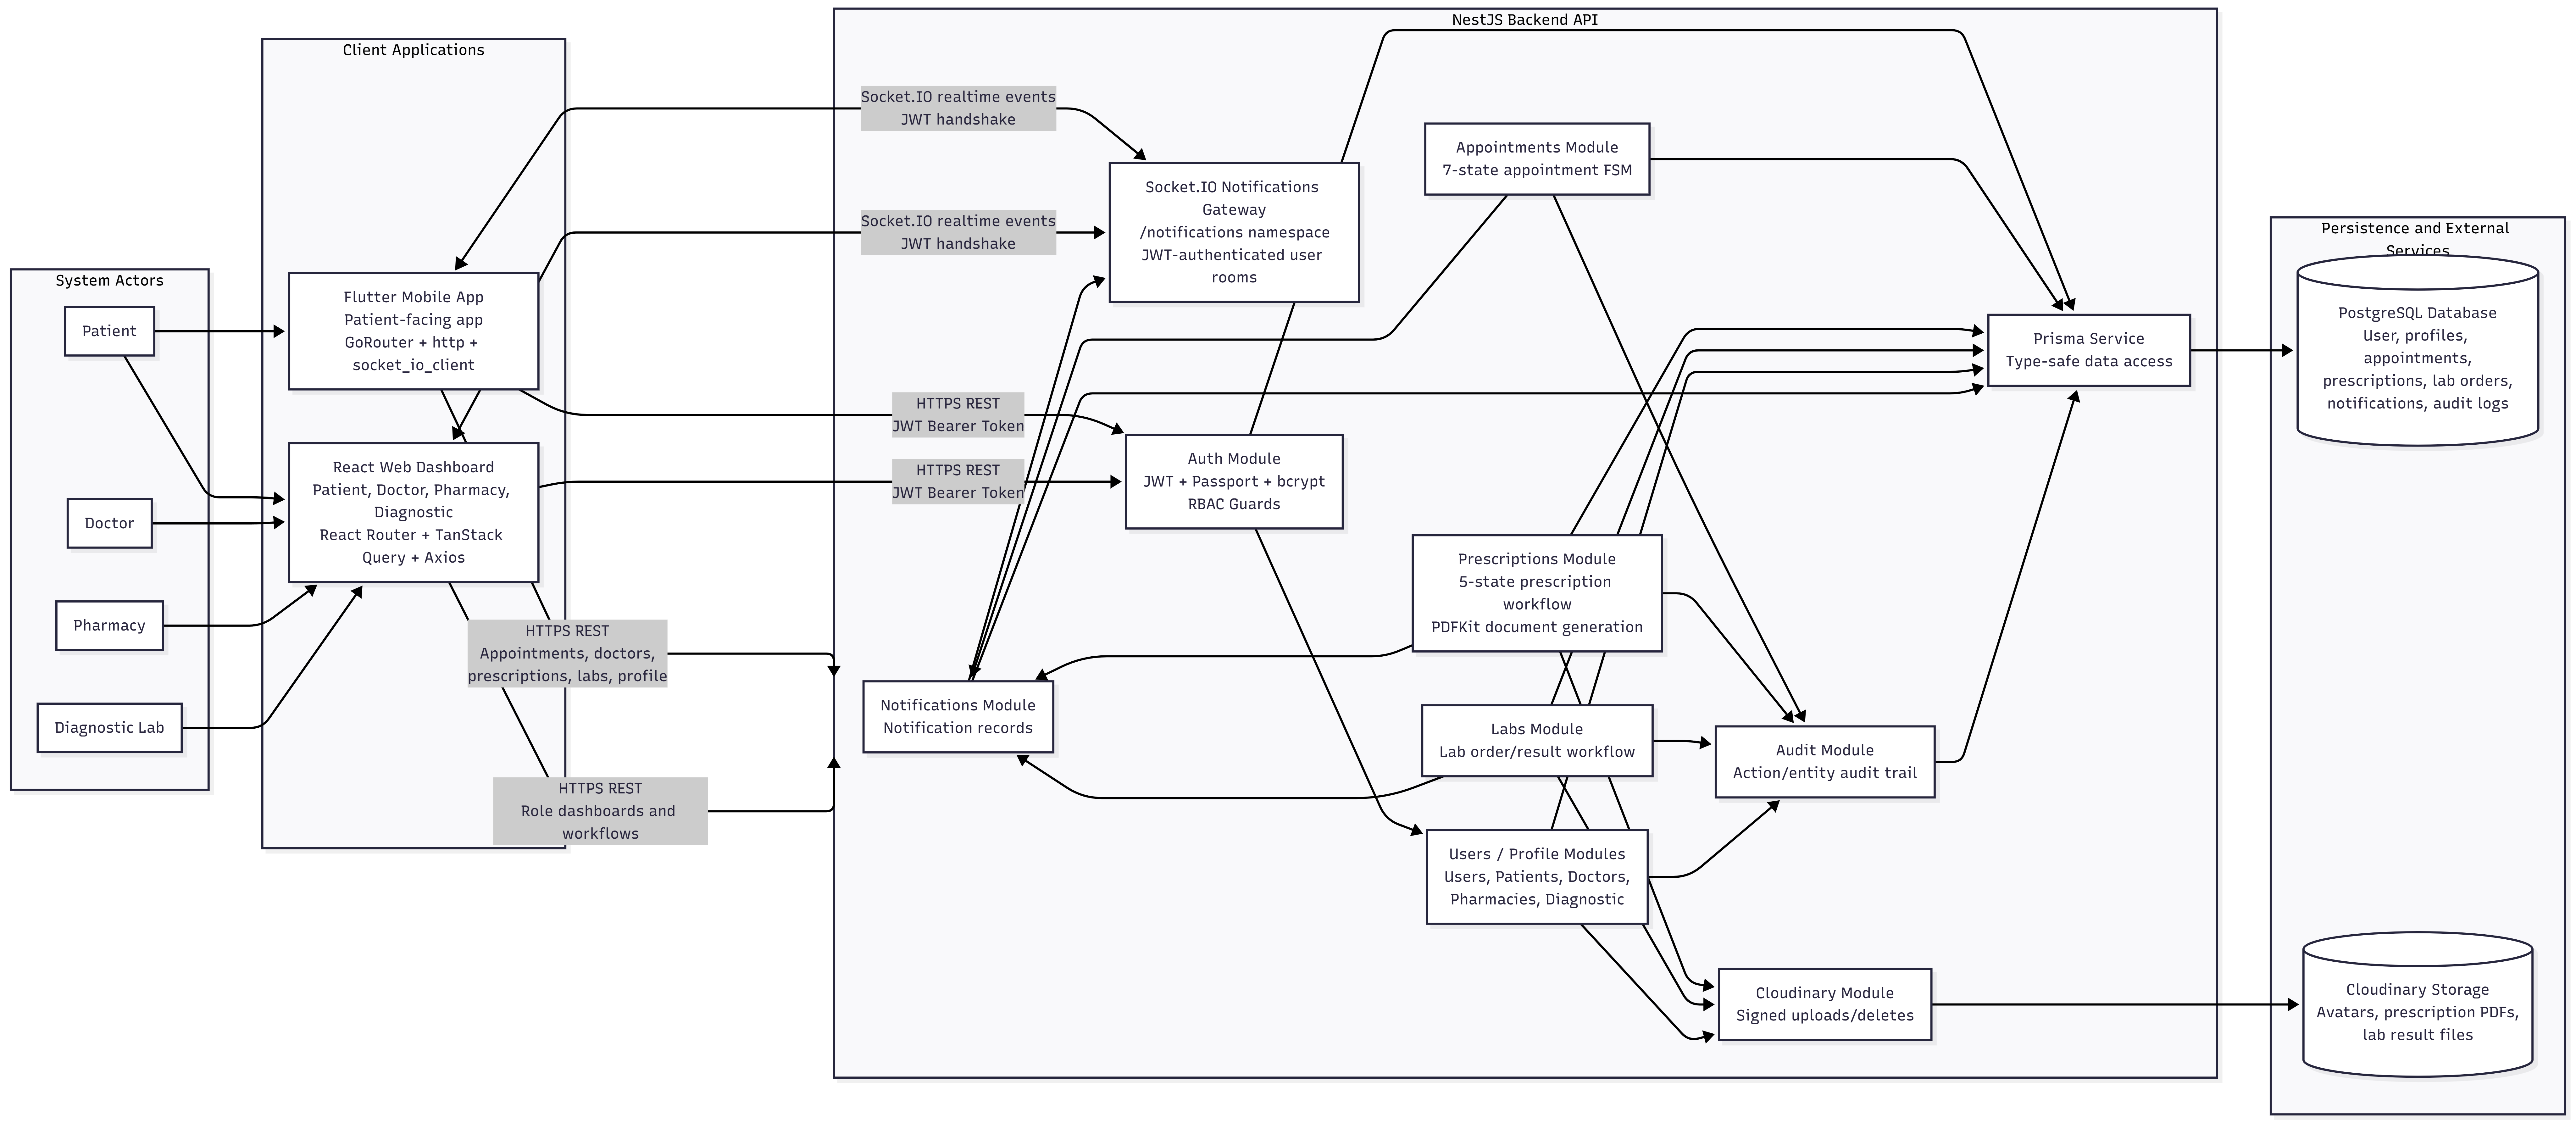
\includegraphics[width=0.78\textheight,height=0.92\textwidth,keepaspectratio]{architecture-diagram}}
\caption{Overall System Architecture of MedFlow}
\label{fig:arch}
\end{figure}

The system is based on three-tier architecture. The \textbf{Presentation Tier} holds:
the React web SPA and Flutter mobile app, both based on REST and Socket.IO. The
 \textbf{Application Tier} This is the NestJS routing, authentication and business server.
logic, FSM enforcement, PDF generation, file upload coordination. The \textbf{Data
Tier} relies on PostgreSQL using Prisma and Cloudinary avatars, prescription PDFs, and.
lab result files.

\subsection{Data Flow Diagram}

The data flow diagram at level-0 of MedFlow is given in Figure~\ref{fig:dfd0}.
communication between the external actors and the overall MedFlow system boundary.

\begin{figure}[p]
\centering
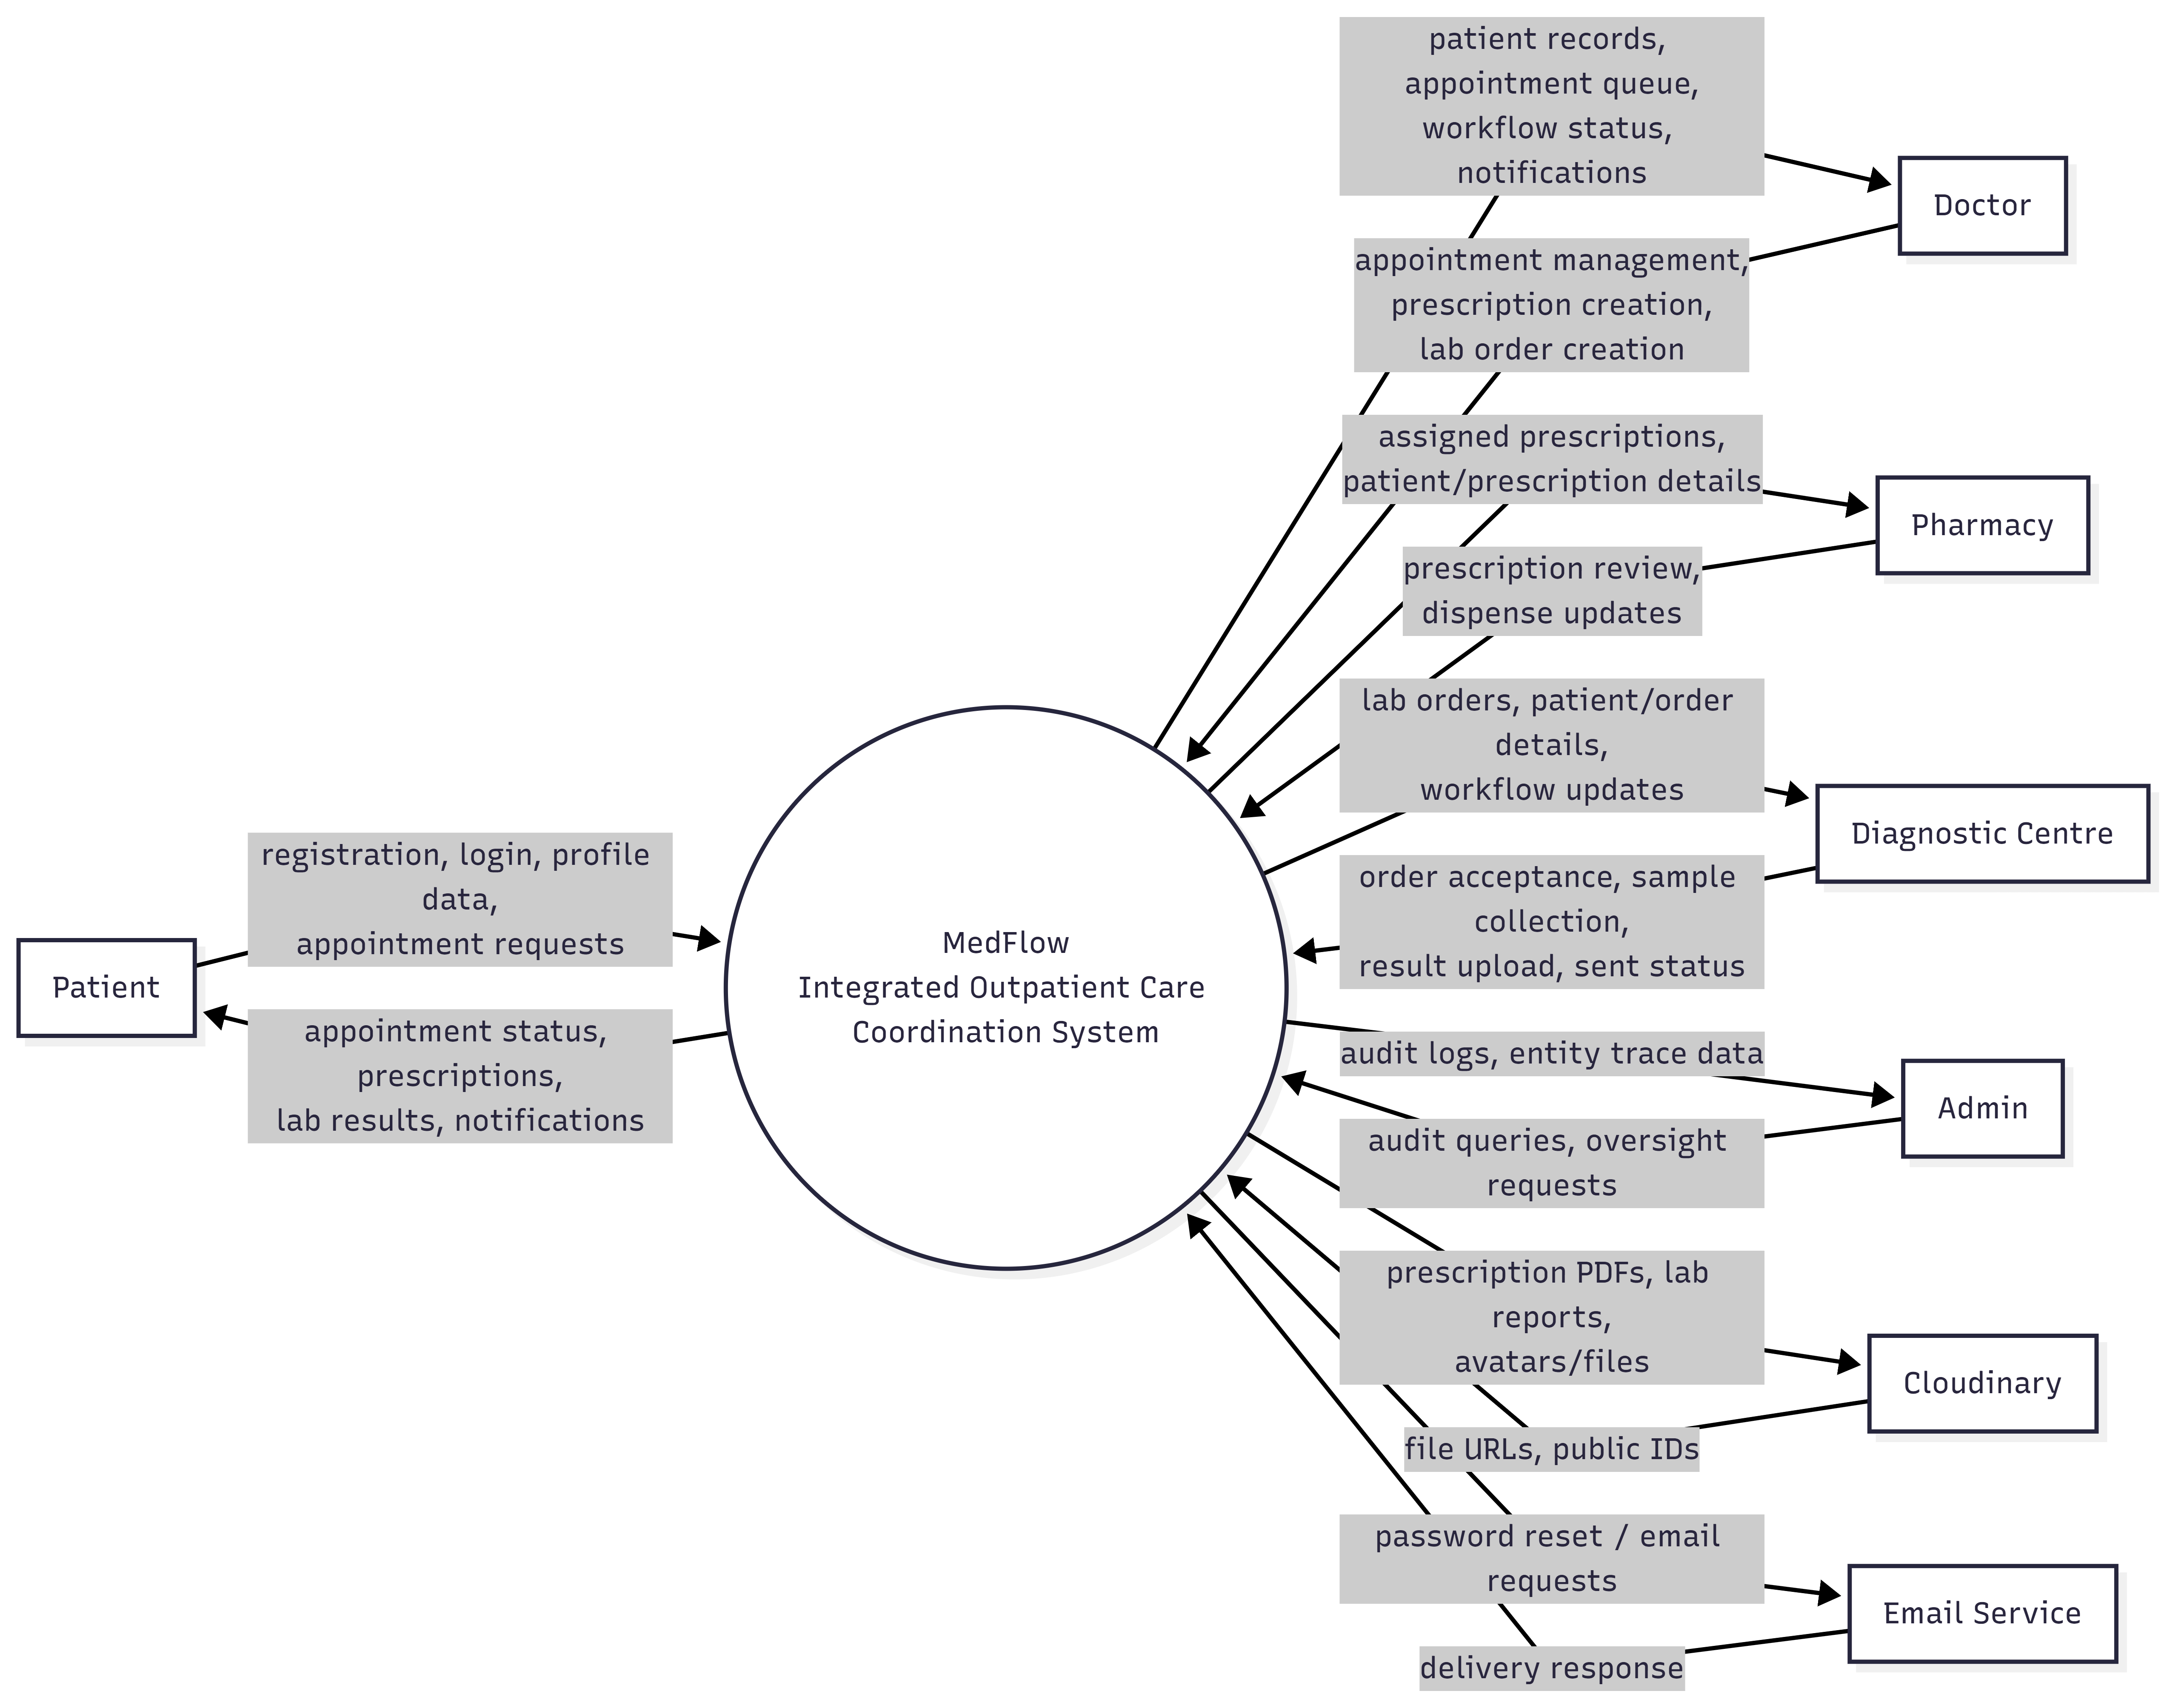
\includegraphics[width=0.95\textwidth,height=0.78\textheight,keepaspectratio]{dfd-level-0}
\caption{Level-0 Data Flow Diagram of MedFlow}
\label{fig:dfd0}
\end{figure}

The data flow diagram at level-1 of MedFlow is given in Figure~\ref{fig:dfd}.
communication between external actors, key application processes, long-lasting data stores,
and email/external file services.

\begin{figure}[p]
\centering
\rotatebox{90}{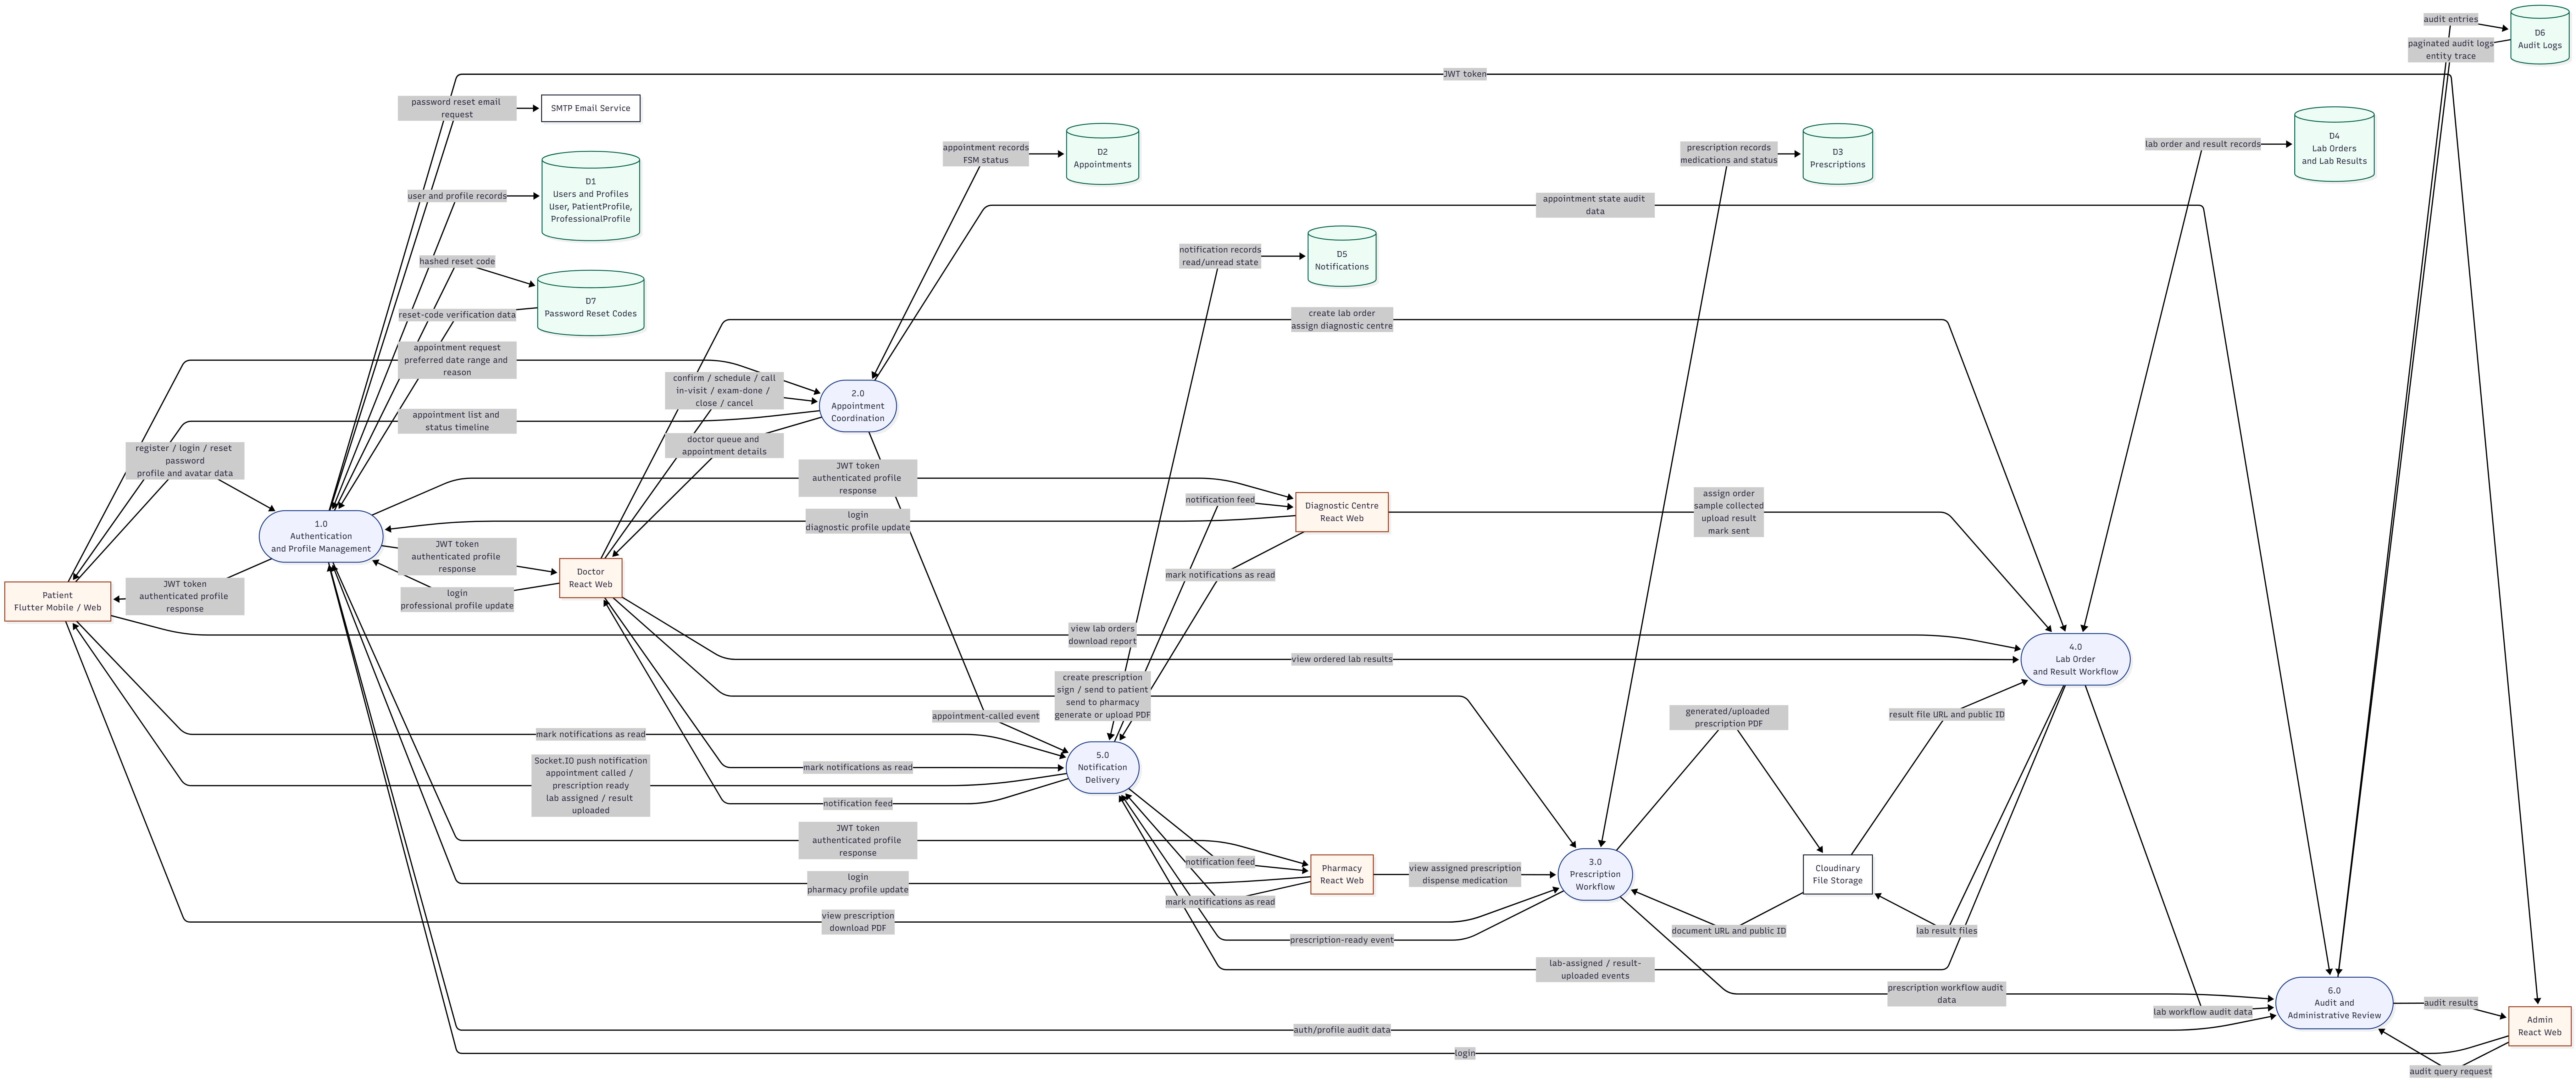
\includegraphics[width=0.78\textheight,height=0.92\textwidth,keepaspectratio]{dfd-level-1}}
\caption{Level-1 Data Flow Diagram of MedFlow}
\label{fig:dfd}
\end{figure}

\subsection{Backend Module Structure}

The NestJS application is structured to have fourteen feature modules each having a distinct encapsulation.
service and DTOs of its own. These modules are summarised in Table~\ref{tab:modules}.
and their responsibilities.

\begin{table}[tbp]
\caption{NestJS Backend Module Structure}
\label{tab:modules}
\centering
\begin{tabular}{|p{3.5cm}|p{9cm}|}
\hline
\textbf{Module} & \textbf{Responsibility}\\
\hline
PrismaModule       & Wraps PrismaClient as a globally injectable singleton service.\\
\hline
CloudinaryModule   & Wraps Cloudinary upload API; provides base64 fallback in development.\\
\hline
HealthModule       & Exposes a \texttt{GET /health} liveness endpoint.\\
\hline
AuthModule         & Registration, login, forgot-password, reset-password, JWT issuance, JwtAuthGuard, RolesGuard.\\
\hline
UsersModule        & User lookup and admin-facing user management endpoints.\\
\hline
PatientsModule     & Patient profile CRUD, doctor search, and avatar upload.\\
\hline
DoctorsModule      & Doctor profile CRUD, public profile viewing, and available time slot management.\\
\hline
PharmaciesModule   & Pharmacy profile CRUD.\\
\hline
DiagnosticModule   & Diagnostic centre profile CRUD and accreditation management.\\
\hline
AppointmentsModule & Appointment creation, listing, and FSM state transitions; integrates notification and audit services.\\
\hline
PrescriptionsModule & Prescription draft creation, PDF generation, status transitions, and pharmacy assignment.\\
\hline
LabsModule         & Lab order creation, assignment, sample collection, and result file upload.\\
\hline
NotificationsModule & Notification creation, listing, mark-read; Socket.IO WebSocket gateway for real-time push.\\
\hline
AuditModule        & Audit log recording and admin-facing paginated query endpoint.\\
\hline
\end{tabular}
\end{table}

\subsection{Web Frontend Architecture}

The React web application is based on role-scoped feature folders, \texttt{TanStack Query}, guarded nested routes.
and a Socket.Notification event notification client. Recharts powers the
Weekly patient-growth and appointment charts by doctor dashboard.

\subsection{Mobile Frontend Architecture}

The Flutter application is based on a layered architecture: its \texttt{core/api} layer offers typed REST and
\texttt{core/domain}, multipart calls, define Dart models and enums.
features per patient separates repositories, mappers, controllers, and pages.
\texttt{GoRouter} is declarative navigation based on a persistent \texttt{PatientShell}.
\texttt{Session Controller} is the controller that powers redirects on login. Live updates come in the form of.
\texttt{Computersocketio client} and update the notification centre.

\section{Problem Design and Analysis}

This section includes the problem design and analysis.

\subsection{Role Identification}

Outpatient workflow analysis revealed five types of actors.

\begin{itemize}[leftmargin=0.7in]
  \item \textbf{Patient ---} Signs up with a medical profile, searches the available physicians, books.
        appointment requests, check appointment status, prescription and lab views.
        receives real-time push notifications, results.
  \item \textbf{Doctor ---} Handles an appointment queue, promotion of appointment states, views.
        prescribes, assigns lab, patient medical histories and clinical records.
        sends requests to diagnostic centres, and views an analytics dashboard.
  \item \textbf{Pharmacy ---} Receives prescriptions given by doctors, reads medication de-
        tails, retrieves prescription PDFs and progresses prescription status until.
        dispensing.
  \item \textbf{Diagnostic ---} Takes lab orders assigned by doctors, accepts orders,
        gathers samples, uploads result files on Cloudinary and informing patients when.
        reports are ready.
  \item \textbf{Admin ---} Can access paginated logs and has system-wide administrator privileges.
\end{itemize}

The MedFlow use case diagram is subdivided into four sections that can be read.
Its presentation (Figures~\ref{fig:usecase_1} through \ref{fig:usecase_4} since) is too large to be included within the entire model.
single A4 page.

\begin{figure}[p]
\centering
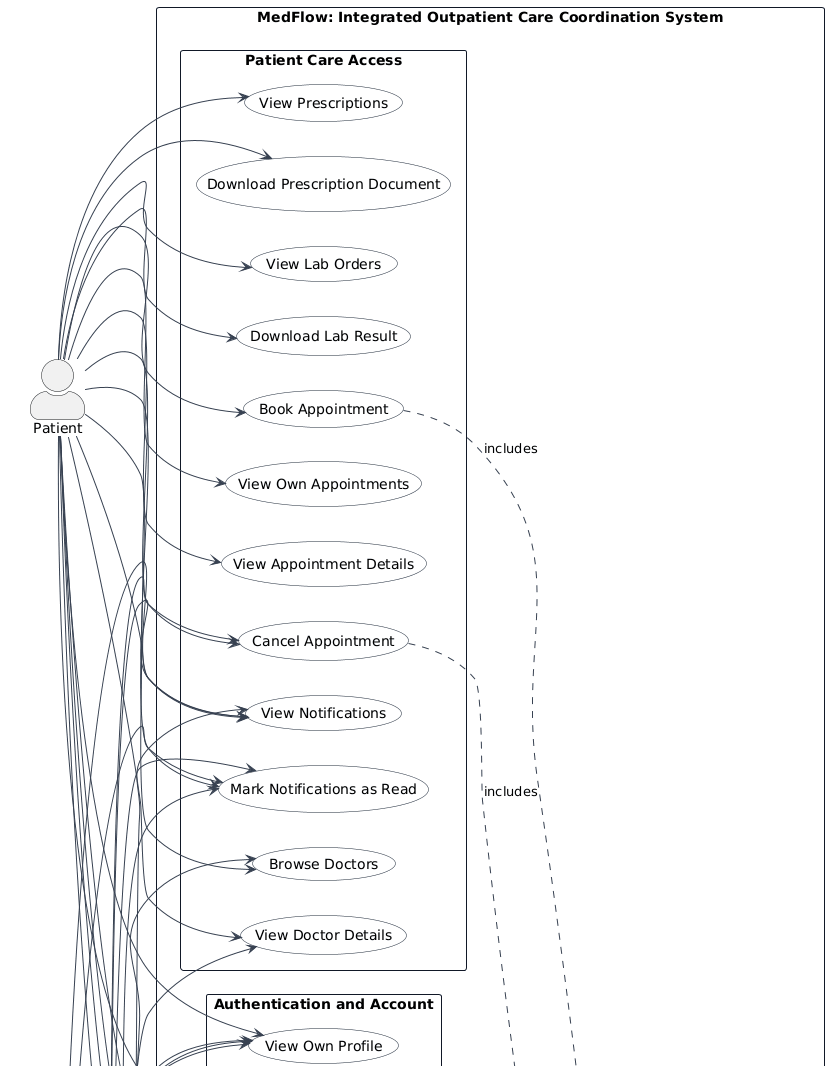
\includegraphics[height=0.78\textheight,keepaspectratio]{use-case-diagram-part-1}
\caption{Use Case Diagram of MedFlow --- Authentication and Patient Care Access}
\label{fig:usecase_1}
\end{figure}

\begin{figure}[p]
\centering
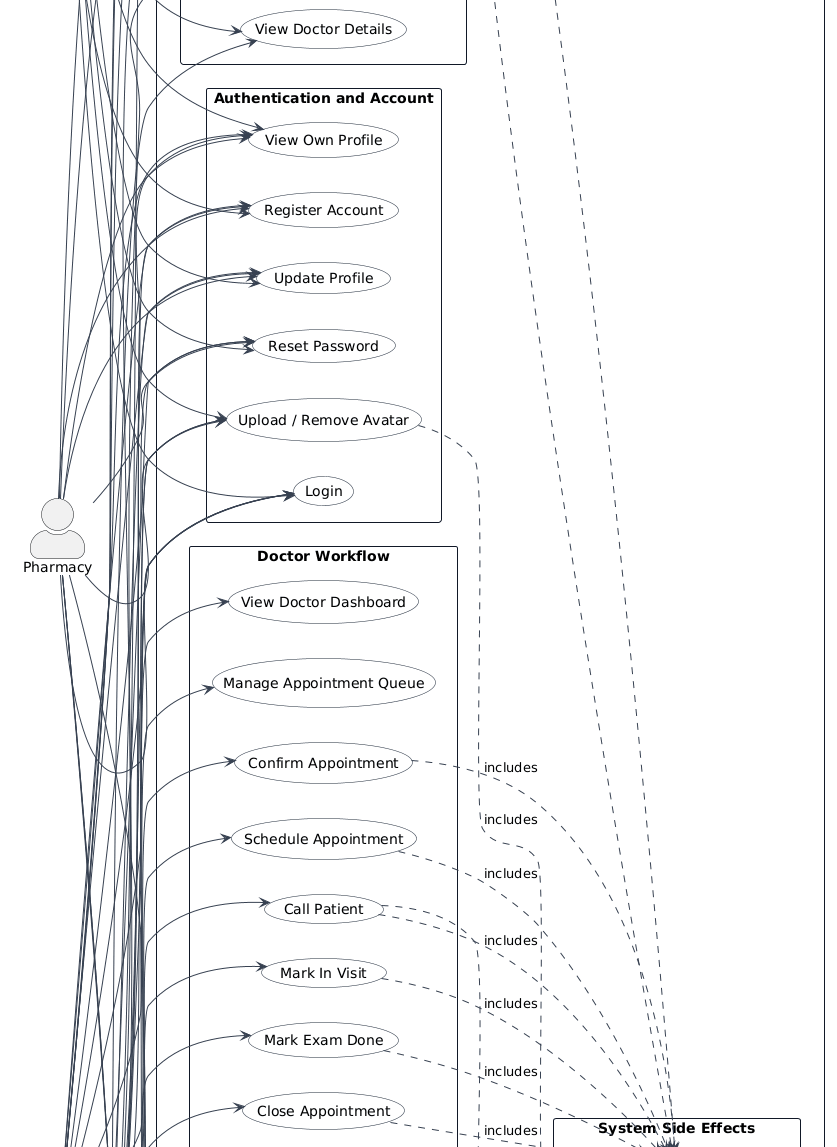
\includegraphics[height=0.78\textheight,keepaspectratio]{use-case-diagram-part-2}
\caption{Use Case Diagram of MedFlow --- Patient and Doctor Workflows}
\label{fig:usecase_2}
\end{figure}

\begin{figure}[p]
\centering
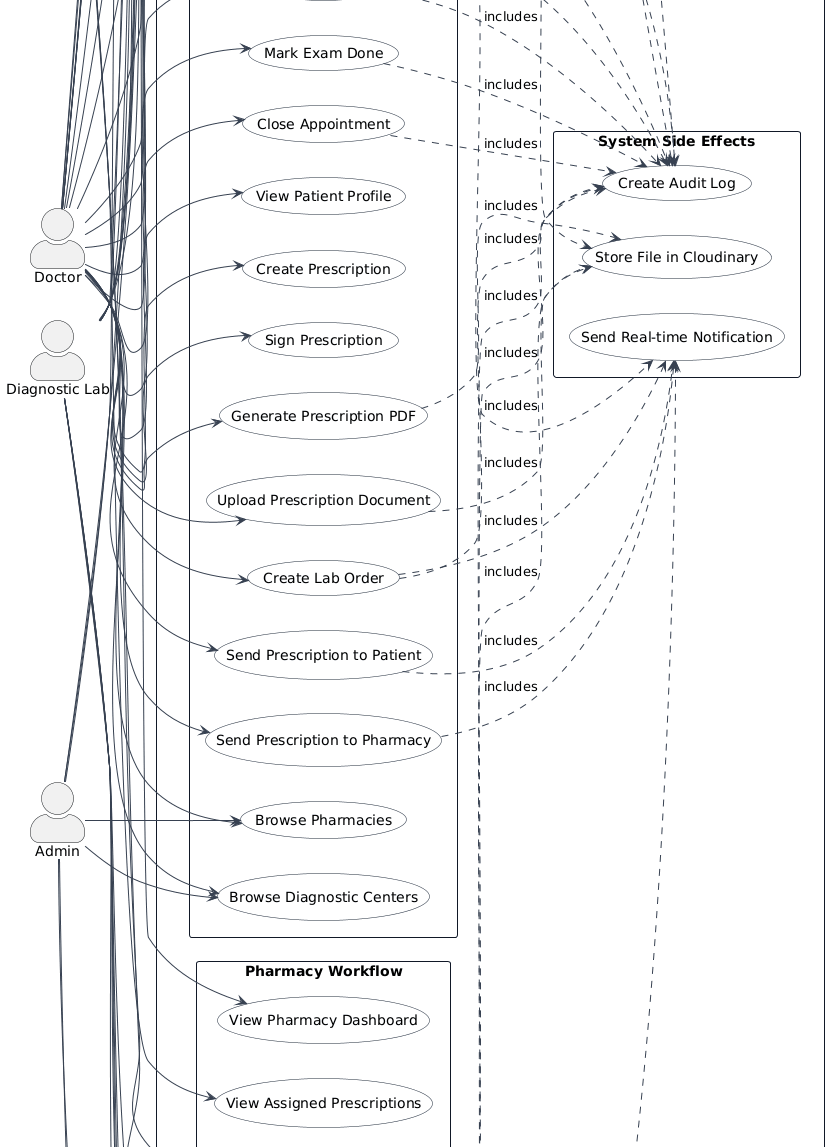
\includegraphics[height=0.78\textheight,keepaspectratio]{use-case-diagram-part-3}
\caption{Use Case Diagram of MedFlow --- Pharmacy and Diagnostic Workflows}
\label{fig:usecase_3}
\end{figure}

\begin{figure}[p]
\centering
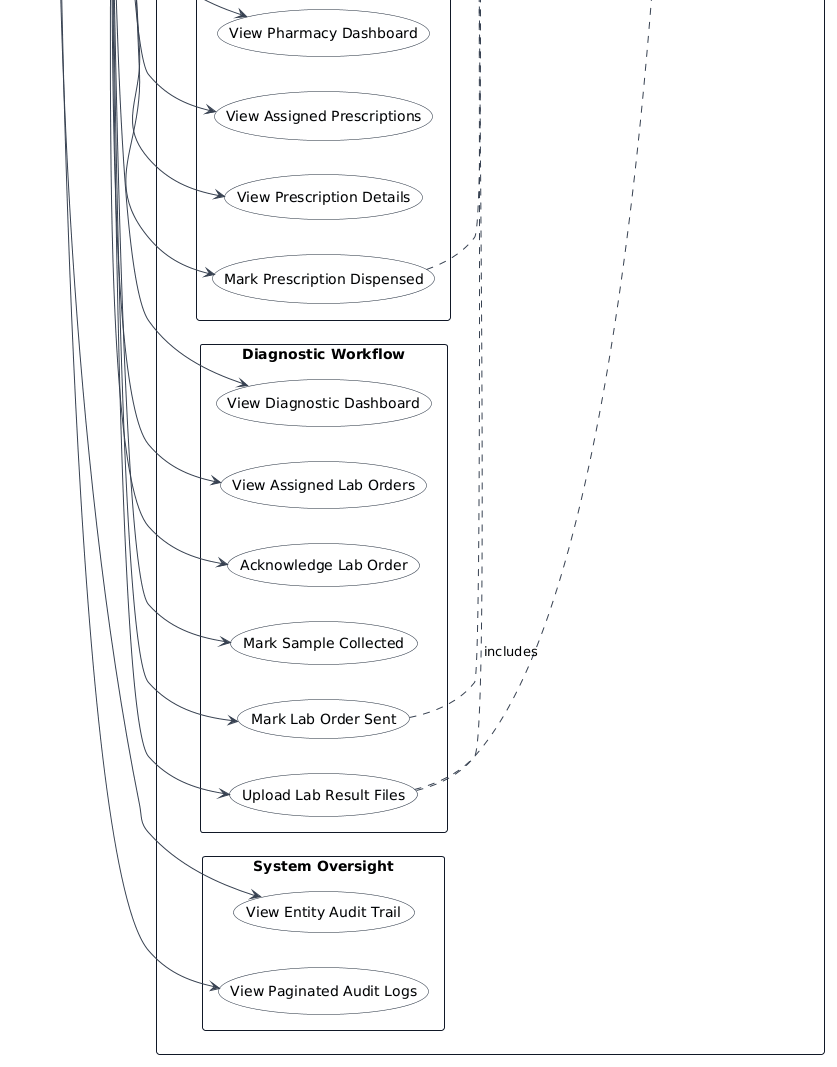
\includegraphics[height=0.78\textheight,keepaspectratio]{use-case-diagram-part-4}
\caption{Use Case Diagram of MedFlow --- Oversight and System Side Effects}
\label{fig:usecase_4}
\end{figure}

\subsection{Appointment State Machine}

The role capability lifecycle was represented by a seven state finite-state machine. Ta-
Each state is defined in ble~\ref{tab:appt_states} and Figure~\ref{fig:appt_fsm} shows the allowed transitions as encoded in.
the program code on the back-end server.

\begin{table}[tbp]
\caption{Appointment States and Clinical Semantics}
\label{tab:appt_states}
\centering
\begin{tabular}{|p{3.2cm}|p{9cm}|}
\hline
\textbf{State}  & \textbf{Semantics}\\
\hline
REQUESTED   & Patient has submitted a request; awaiting doctor confirmation. A preferred date range and a time note may accompany the request.\\
\hline
CONFIRMED   & Doctor has accepted and the appointment is scheduled.\\
\hline
CALLED      & Patient has been called to the waiting area. A push notification is dispatched to the patient at this transition.\\
\hline
IN\_VISIT   & Patient is currently in the consultation room.\\
\hline
EXAM\_DONE  & Consultation is complete. Lab orders and prescriptions may now be created.\\
\hline
CLOSED      & All associated steps are resolved. Appointment is finalised.\\
\hline
CANCELLED   & Appointment was cancelled by patient, doctor, or admin.\\
\hline
\end{tabular}
\end{table}

\begin{figure}[tbp]
\centering
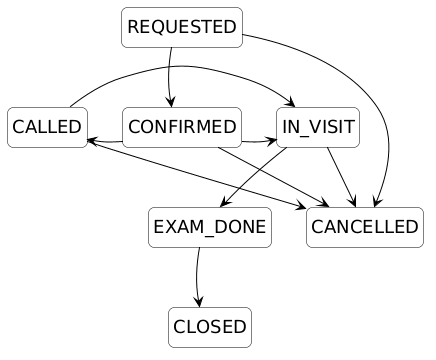
\includegraphics[width=0.95\textwidth,height=0.55\textheight,keepaspectratio]{appointment-fsm}
\caption{Appointment Finite-State Machine}
\label{fig:appt_fsm}
\end{figure}

\subsection{Prescription State Machine}

Prescriptions are an independent five-state lifecycle also reference by a transition.
map of the prescriptions service. Each state is defined in Table~\ref{tab:rx_states}.

\begin{table}[tbp]
\caption{Prescription States and Semantics}
\label{tab:rx_states}
\centering
\begin{tabular}{|p{4.9cm}|p{7.3cm}|}
\hline
\textbf{State}       & \textbf{Semantics}\\
\hline
DRAFT                & Doctor has created the prescription but not yet finalised it.\\
\hline
SIGNED               & Doctor has signed the prescription; the generated PDF document can then be uploaded to Cloudinary.\\
\hline
SENT\_TO\_PATIENT    & Prescription is visible to the patient; a push notification is dispatched.\\
\hline
SENT\_TO\_PHARMACY   & Prescription has been forwarded to the assigned pharmacy.\\
\hline
DISPENSED            & Pharmacy has dispensed the medication; the workflow is complete.\\
\hline
\end{tabular}
\end{table}

\begin{figure}[p]
\centering
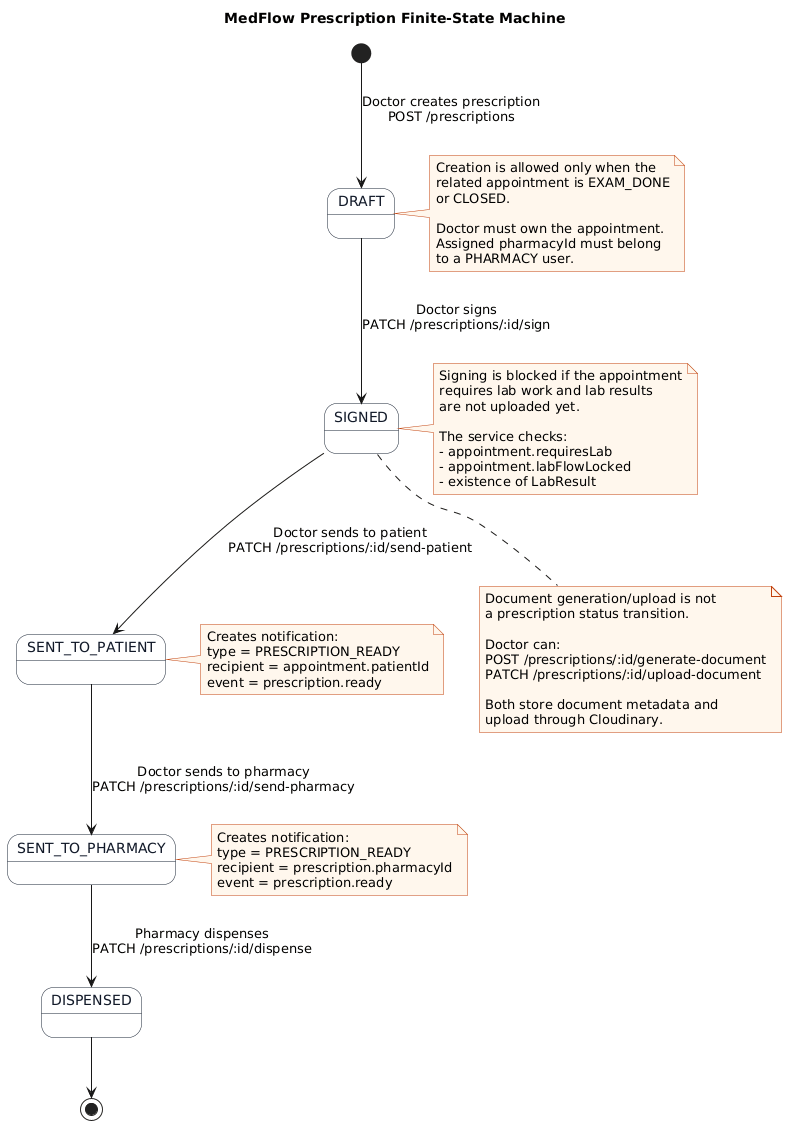
\includegraphics[height=0.78\textheight,keepaspectratio]{prescription-fsm-diagram}
\caption{Prescription Finite-State Machine}
\label{fig:rx_fsm}
\end{figure}

\subsection{Lab Order State Machine}

Orders in Labs have a four-state lifecycle which is categorized in Table~\ref{tab:lab_states}.

\begin{table}[tbp]
\caption{Lab Order States and Semantics}
\label{tab:lab_states}
\centering
\begin{tabular}{|p{3.8cm}|p{8.4cm}|}
\hline
\textbf{State}       & \textbf{Semantics}\\
\hline
CREATED              & Doctor has created the order and assigned a diagnostic centre.\\
\hline
ASSIGNED             & Diagnostic centre has acknowledged the order; push notification dispatched to patient.\\
\hline
SAMPLE\_\allowbreak COLLECTED    & Diagnostic centre has collected the biological sample.\\
\hline
SENT                 & Result file uploaded to Cloudinary; push notification dispatched; patient may now download the report.\\
\hline
\end{tabular}
\end{table}

\begin{figure}[p]
\centering
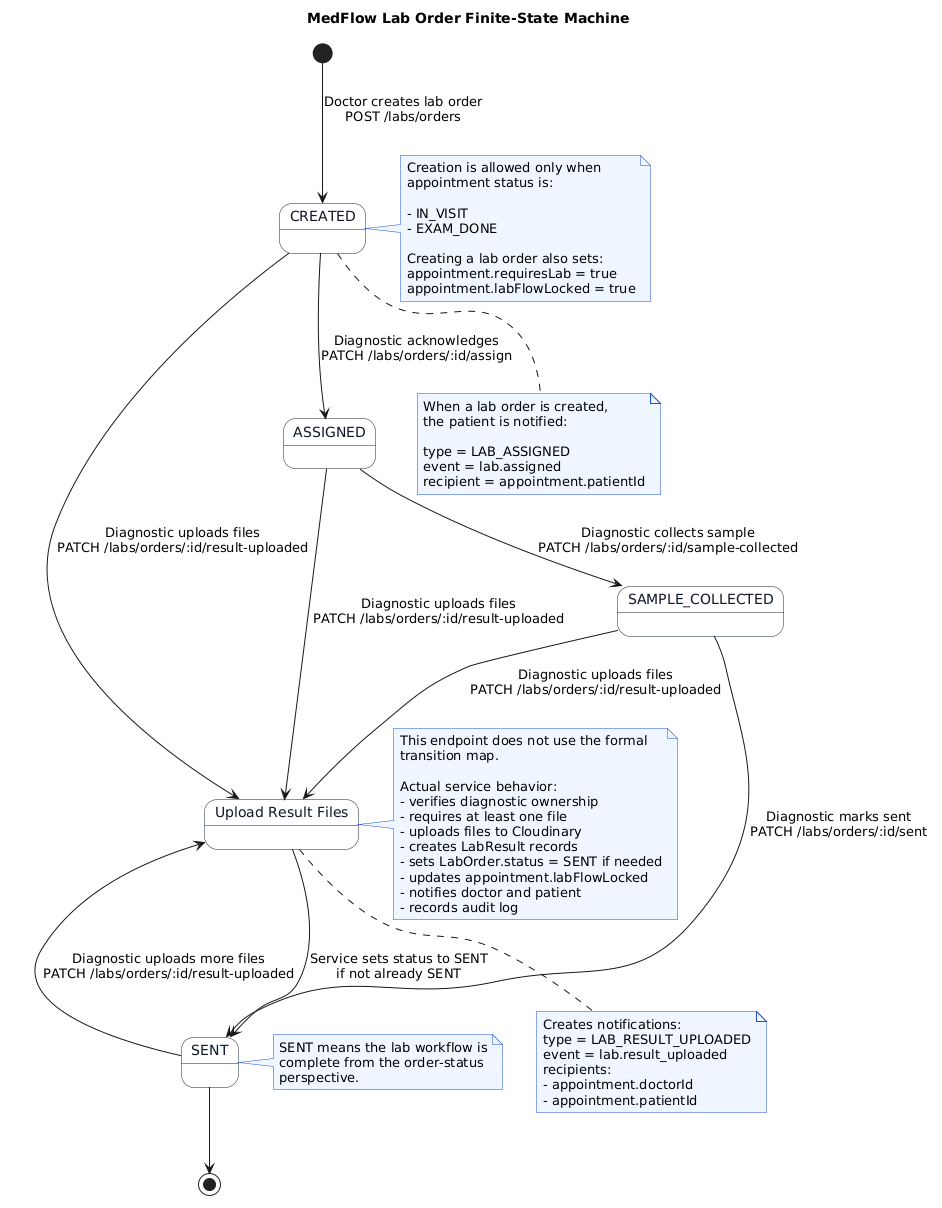
\includegraphics[height=0.78\textheight,keepaspectratio]{lab-order-fsm-diagram}
\caption{Lab Order Finite-State Machine}
\label{fig:lab_fsm}
\end{figure}

\section{Database Schema Design}

There are ten Prisma schema models. An overall projection of is given in Table~\ref{tab:schema}.
if it has a model, its essential fields, and relationships.

\begin{table}[tbp]
\caption{Database Schema --- Model Overview}
\label{tab:schema}
\centering
\begin{tabular}{|p{3.2cm}|p{9cm}|}
\hline
\textbf{Model} & \textbf{Key Fields and Relationships}\\
\hline
User               & UUID PK, fullName, avatarUrl, email (unique), passwordHash, role (enum), phone, address; relates to PatientProfile, ProfessionalProfile, Appointments (as patient and doctor), LabOrders (as diagnostic), Prescriptions (as doctor and pharmacy), Notifications, AuditLogs, PasswordResetCodes.\\
\hline
PatientProfile     & One-to-one with User; stores dateOfBirth, gender, allergies, chronicConditions, currentMedications, and emergency contact fields.\\
\hline
ProfessionalProfile & One-to-one with User; stores licenseNumber, specialization, about, clinicName, clinicAddress, availableTimeSlots (JSON), degrees (JSON), certifications (JSON), yearsOfExperience, availableTests (JSON); fields used selectively based on role.\\
\hline
Appointment        & UUID PK; patientId and doctorId FKs to User; status (AppointmentStatus enum); scheduledAt, reason, preferredDateFrom, preferredDateTo, preferredTimeNote, requiresLab, labFlowLocked; relates to LabOrders and Prescriptions.\\
\hline
LabOrder           & UUID PK; appointmentId FK; diagnosticId FK to User; status (LabOrderStatus enum); tests (JSON array); relates to LabResults.\\
\hline
LabResult          & UUID PK; labOrderId FK; fileUrl, filePublicId, fileMimeType, fileSizeBytes; uploadedAt timestamp.\\
\hline
Prescription       & UUID PK; appointmentId FK; doctorId and pharmacyId FKs to User; notes, diagnosis, instructions, medications (JSON); status (PrescriptionStatus enum); documentUrl, documentPublicId, documentVersion.\\
\hline
Notification       & UUID PK; userId FK; type (NotificationType enum: APPOINTMENT\_CALLED, LAB\_ASSIGNED, LAB\_RESULT\_UPLOADED, PRESCRIPTION\_READY); message; read boolean.\\
\hline
AuditLog           & UUID PK; actorUserId FK; action, entityType, entityId strings; metadata (JSON); createdAt.\\
\hline
PasswordResetCode  & UUID PK; userId FK; email; codeHash (SHA-256); expiresAt; consumedAt; attemptCount; rate-limited to 5 attempts.\\
\hline
\end{tabular}
\end{table}

The entity relationships that were produced based on the real Prisma schema are displayed in Figure~\ref{fig:er_diagram}.

\begin{figure}[p]
\centering
\includegraphics[width=0.95\textwidth,height=0.78\textheight,keepaspectratio]{er-diagram}
\caption{Entity Relationship Diagram of MedFlow}
\label{fig:er_diagram}
\end{figure}

\section{Conclusion}

The decision-making process of the system analysis and design remained based on outpatient work-.
flows. Prisma is the source of truth on the data-layer, and NestJS modules are modules on the backend.
concerns, and the web and mobile clients have equal API contract via TypeScript.
and Dart models.

% ============================================================
%  CHAPTER IV -- IMPLEMENTATION, RESULTS AND DISCUSSIONS
% ============================================================
\chapter{Implementation, Results and Discussions}
\label{chap:implementation-results-and-discussions}

\section{Introduction}

The chapter includes implementation, API design, the frontend structure, and test.
outcomes within the three components of the applications.

\section{Experimental Setup}

Components were created and tested on Ubuntu 22.04 LTS with Node.js.
v20, npm 10, NestJS CLI 11, Prisma CLI 7, PostgreSQL in Docker, TypeScript 5.9,
Flutter/Dart, Vite, Vitest with Testing Library, and Flutter Test: 3.11.

\section{Evaluation Metrics}

Assessment included correctness of backend services/controllers, and role enforcement, FSM.
integrity, dispatches notification to asserted rooms and schema-level data integrity and
role-gated page behaviour, loading behaviour, and error behaviour.

\section{Dataset}

Synthetic test data has been developed using \texttt{backend/prisma/seed.ts}. It includes
Product features (and URLs) patient and professional profiles, appointments, prescriptions, lab
orders, lab results, and notifications, giving a realistic foundation of manual and automated.
testing.

\section{Implementation and Results}

\subsection{Backend Implementation}

\subsubsection{Authentication and Registration}

Registration takes one role specific profile data request. Patients submit medical
although professional profile is submitted by doctors, pharmacies, and diagnostic users, profile fields.
fields. \texttt{bcrypt} is used to hash passwords, and the login provides a JWT with user UUID,
email, and role. A six-digit code that is stored in the password reset flow as a hash of \texttt{SHA-256}.
protecting expiry, attempt limiting and consumed state.

\subsubsection{Appointment Service}

The appointment service puts a list of allowed transitions in a look up table (Listing~\ref{lst:transitions}).
Trigger transitions, like \texttt{CALLED}, do not reset the state, but send out a \texttt{Socket.IO}
cast to authenticated room of patient.

\begin{lstlisting}[language=TypeScript,caption={Appointment FSM Transition Map},label={lst:transitions}]
const TRANSITIONS: Record<AppointmentStatus, AppointmentStatus[]> = {
  REQUESTED: [CONFIRMED, CANCELLED],
  CONFIRMED: [CALLED, IN_VISIT, CANCELLED],
  CALLED:    [IN_VISIT, CANCELLED],
  IN_VISIT:  [EXAM_DONE, CANCELLED],
  EXAM_DONE: [CLOSED],
  CLOSED:    [],
  CANCELLED: [],
};
\end{lstlisting}

\subsubsection{Prescription Service}

Only when the appointment is \texttt{EXAM\_DONE} or less, it can create prescriptions.
\texttt{CLOSED}. Physicians put signatures on prescriptions, create or upload PDF files using Cloudinary,
and forwards the prescription FSM. Once a prescription is sent to \texttt{SENT\_TO\_PATIENT}, a \texttt{PRESCRIPTION\_READY} notification is sent.

\subsubsection{Lab Order and Result Service}

Lab orders are developed by doctors and include a diagnostic centre and requested tests. \texttt{ASSIGNED}
and \texttt{SENT} transition informs the patient; uploading of the result means saving the file in Cloudinary and
develops a \texttt{LabResult} record.

\subsubsection{WebSocket Notification Gateway}

All Sockets are authenticated by the \texttt{NotificationsGateway} \texttt{Socket.IO} connection with
Join to \texttt{user:} joins it to \texttt{user:\{userId\}}. Emits: services call \texttt{emitToUser(userId, event,}
\texttt{payload)} to only broadcast to that room; spoisy tokens have their connection cut off.

Figure~\ref{fig:appointment_notification_sequence} illustrates a sequence that was implemented to further advance an appointment to \texttt{CALLED},
authorization, transition validation, notification persistence, \texttt{Socket.IO} emission,
and audit logging.

\begin{figure}[p]
\centering
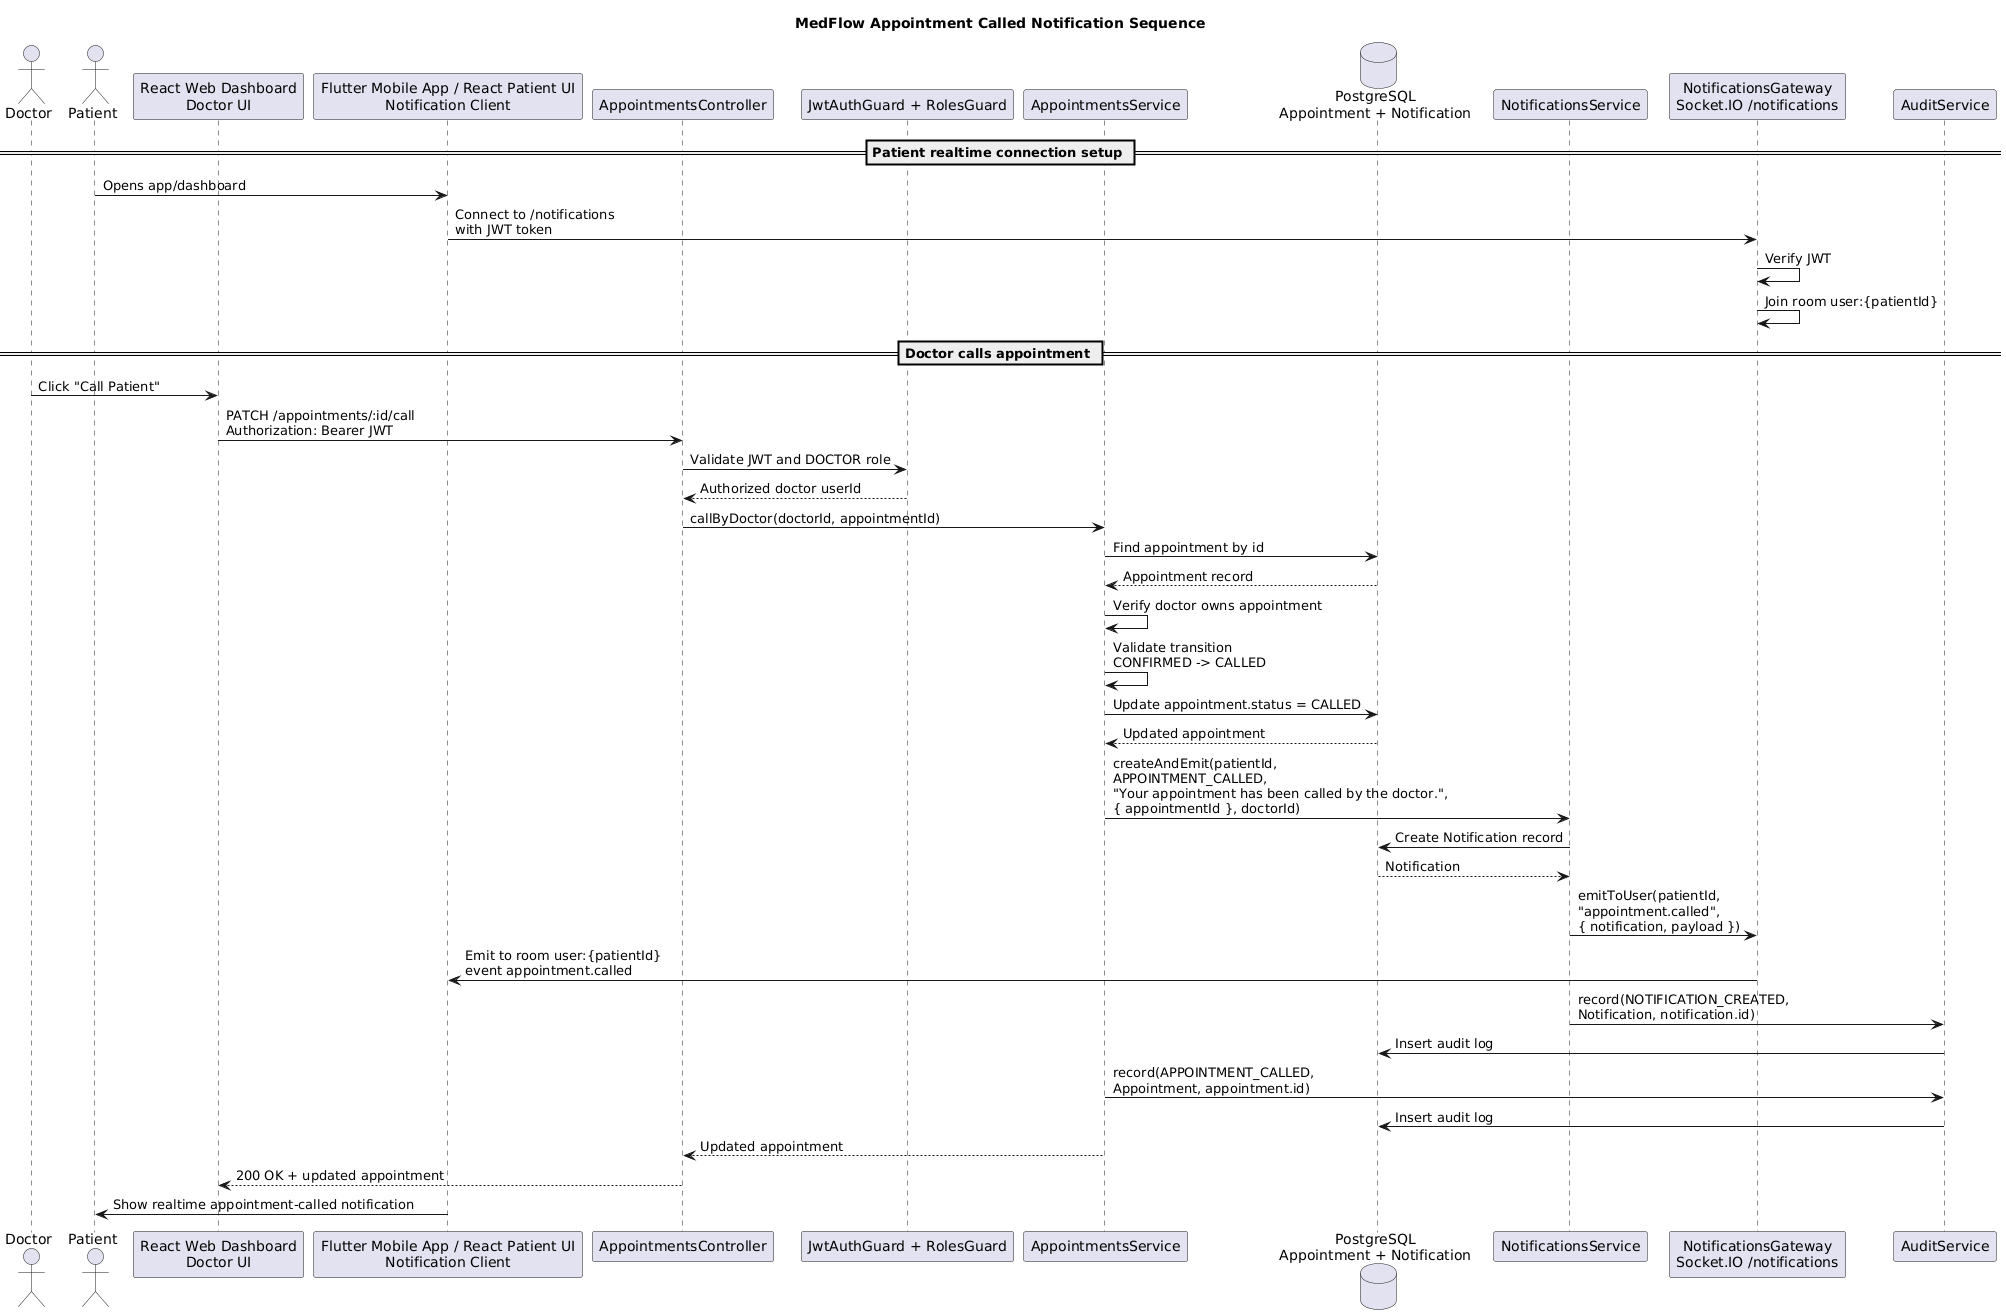
\includegraphics[width=0.95\textwidth,height=0.78\textheight,keepaspectratio]{appointment-notification-sequence-diagram}
\caption{Appointment Called Notification Sequence}
\label{fig:appointment_notification_sequence}
\end{figure}

\subsubsection{Cloudinary Service}

The \texttt{CloudinaryService} encrypts upload requests using \texttt{HMAC-SHA256} and re-encrypts the uploads.
appendages the URL, public ID, version, MIME type and the size of the bytes. Without Cloudinary credentials,
it provides a base64 data URI to allow development processes to continue.

\subsection{REST API Endpoints}

The major API groups are summarised in Table~\ref{tab:endpoints}. Specific transition is revealed through controllers.
endpoints, rather than a generic endpoint in the status of workflows, where invalid changes of any workflow may be.
rejected clearly.

\begin{table}[tbp]
\caption{Principal REST API Endpoint Groups}
\label{tab:endpoints}
\centering
\footnotesize
\setlength{\tabcolsep}{3pt}
\renewcommand{\arraystretch}{1.12}
\begin{tabular}{|p{2cm}|p{5.7cm}|p{2.2cm}|p{2.4cm}|}
\hline
\textbf{Area} & \textbf{Representative Paths} & \textbf{Roles} & \textbf{Purpose}\\
\hline
Authentication & /auth/register, /auth/login, /auth/forgot-password, /auth/reset-password & Public & Registration, JWT login, and password reset.\\
\hline
Appointments & /appointments, /appointments/me, /appointments/:id/confirm, /schedule, /call, /in-visit, /exam-done, /close, /cancel & Patient, Doctor & Booking and appointment FSM transitions.\\
\hline
Prescriptions & /prescriptions, /prescriptions/:id/sign, /send-patient, /send-pharmacy, /dispense, /upload-document, /generate-document & Doctor, Pharmacy & Prescription lifecycle, PDF generation, and dispensing.\\
\hline
Lab Orders & /labs/orders, /labs/orders/me, /labs/orders/:id/assign, /sample-collected, /result-uploaded, /sent, /result & Doctor, Diagnostic, Patient & Lab order creation, diagnostic workflow, and result access.\\
\hline
Notifications & /notifications/me, /notifications/me/read & All authenticated users & Notification listing and read-state updates.\\
\hline
Profiles & /users/doctors, /users/me/avatar, /doctors/me/profile & Patient, Doctor, all authenticated users & Doctor browsing and profile/avatar management.\\
\hline
Audit & /audit, /audit/me, /audit/entity/:entityType/:entityId & Admin, authenticated users & Paginated audit review and entity-specific traces.\\
\hline
\end{tabular}
\end{table}

\subsection{React Web Frontend Implementation}

The web-based system has specific dashboards to display Patient, Doctor, Pharmacy.
and Diagnostic roles. \texttt{RoleHomeRedirect} redirects every user to the appropriate home route after going through the login. Table~\ref{tab:web_pages} is a summary of pages implemented.

\begin{table}[tbp]
\caption{React Web Frontend Pages by Role}
\label{tab:web_pages}
\centering
\begin{tabular}{|p{2.4cm}|p{10cm}|}
\hline
\textbf{Role} & \textbf{Pages Implemented}\\
\hline
Patient    & Appointments list, Appointment details (status timeline, prescription cards, lab order cards), Doctor details, Notifications, Medical records, Profile with avatar upload.\\
\hline
Doctor     & Home dashboard (weekly appointment bar chart, patient growth line chart, recent activity feed), Appointments list and detail, Patient list and individual patient profile, Prescriptions, Lab orders, Notifications, Profile.\\
\hline
Pharmacy   & Home, Prescriptions list, Prescription detail (medication table, download PDF), Notifications, Profile.\\
\hline
Diagnostic & Home, Lab orders list, Lab order detail (test list, upload result file), Notifications, Profile.\\
\hline
\end{tabular}
\end{table}

Appointments, lab orders, prescriptions and notifications are loaded by Doctor home page.
Connects to \texttt{TanStack Query}, and visualizes weekly appointment and patient-growth analytics.
using Recharts.

\begin{figure}[tbp]
\centering
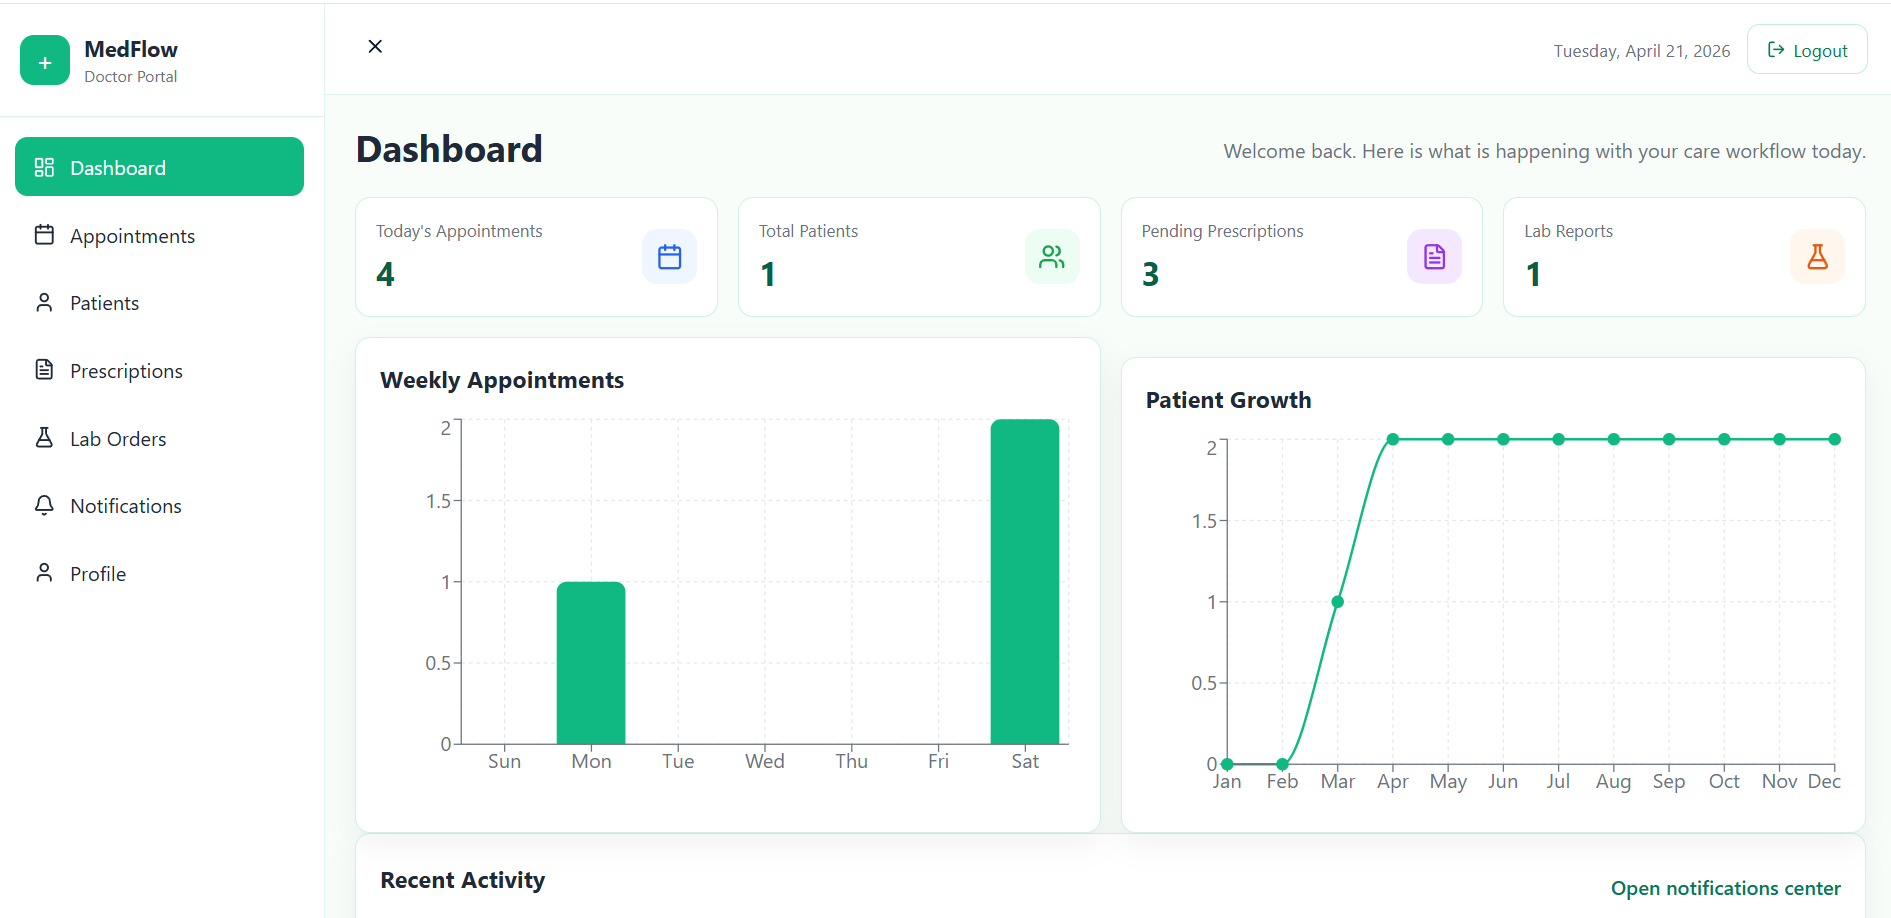
\includegraphics[width=0.95\textwidth,keepaspectratio]{doctor-dashboard}
\caption{Doctor Dashboard and Analytics Interface}
\label{fig:doctor_dashboard}
\end{figure}

\begin{figure}[tbp]
\centering
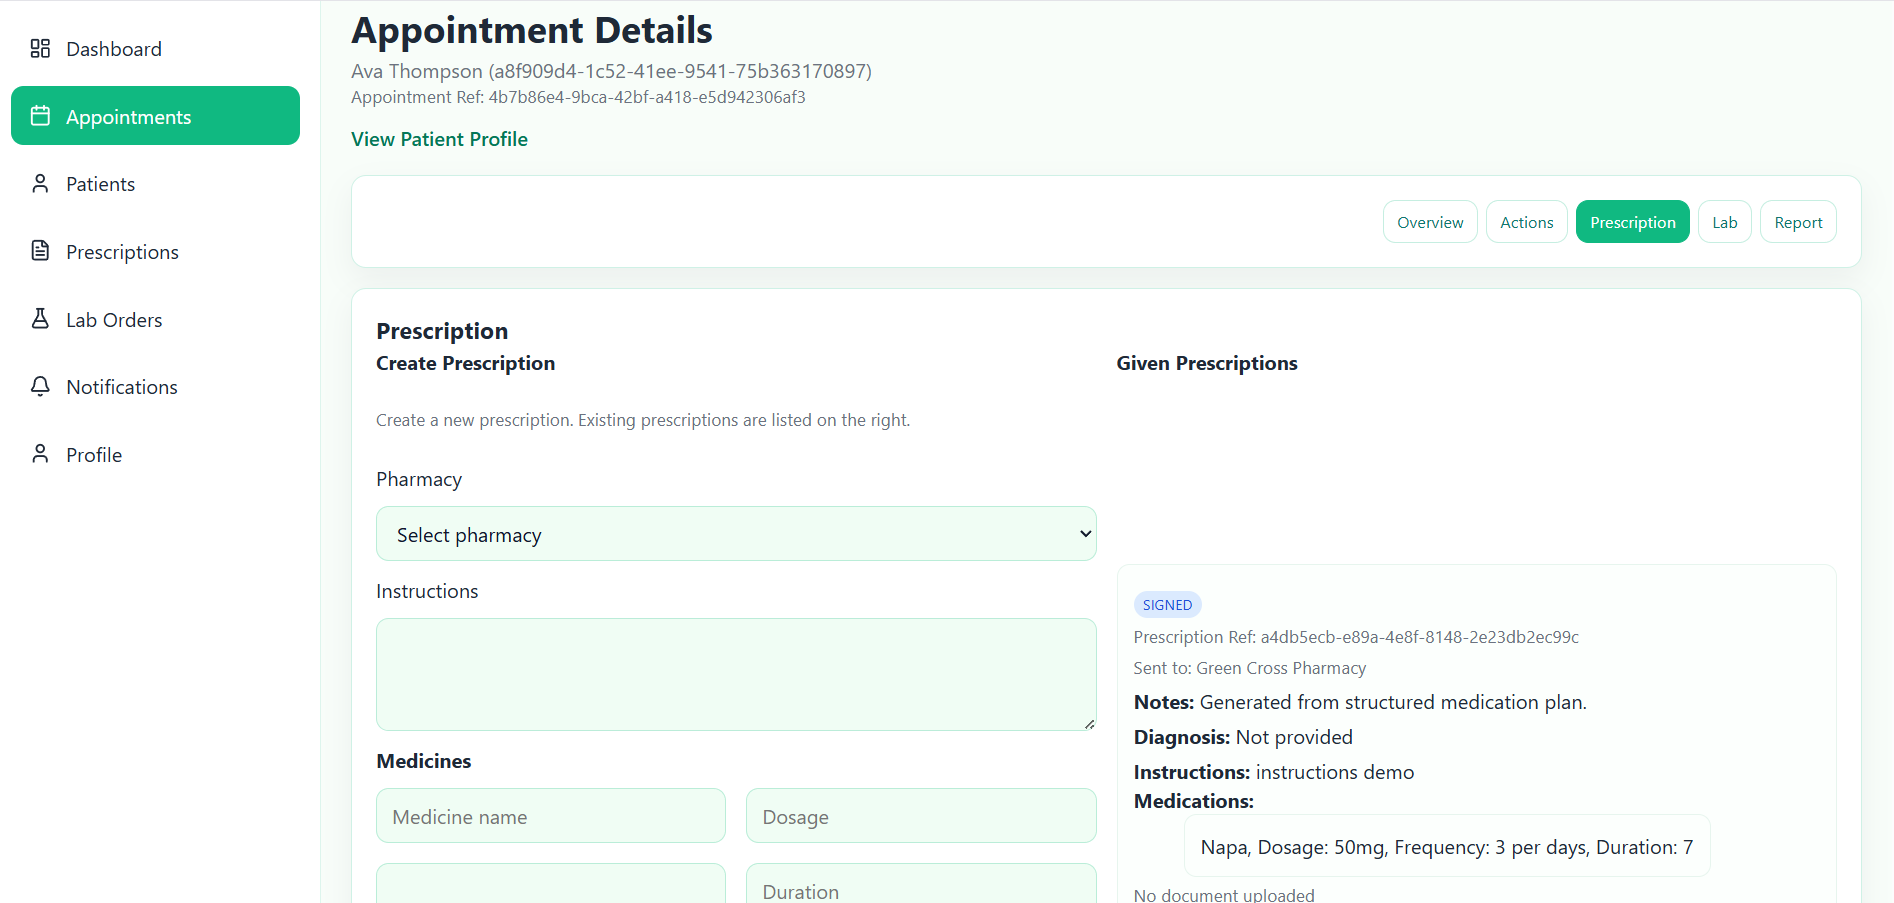
\includegraphics[width=0.95\textwidth,keepaspectratio]{doctor-appointment-details-with-prescription-creation}
\caption{Doctor Appointment Details and Prescription Creation Interface}
\label{fig:doctor_appointment_details}
\end{figure}

\subsection{Flutter Mobile Frontend Implementation}

The Flutter application has the implication of the patient journey: authentication, doctor brows-
ing, making appointments, appointment information, prescription and report downloads, medical.
notifications, management of records and profile/avatar. Listo \texttt{GoRouter} and \texttt{PatientShell} pro-
vide guarded navigating and a bottom persistent bar, with the JWT being stored in \texttt{SessionController} and redirects being triggered. Real-time messages update the unread number using.
\texttt{NotificationsRealtimeService} and \texttt{NotificationsCenterController}.

\begin{figure}[tbp]
\centering
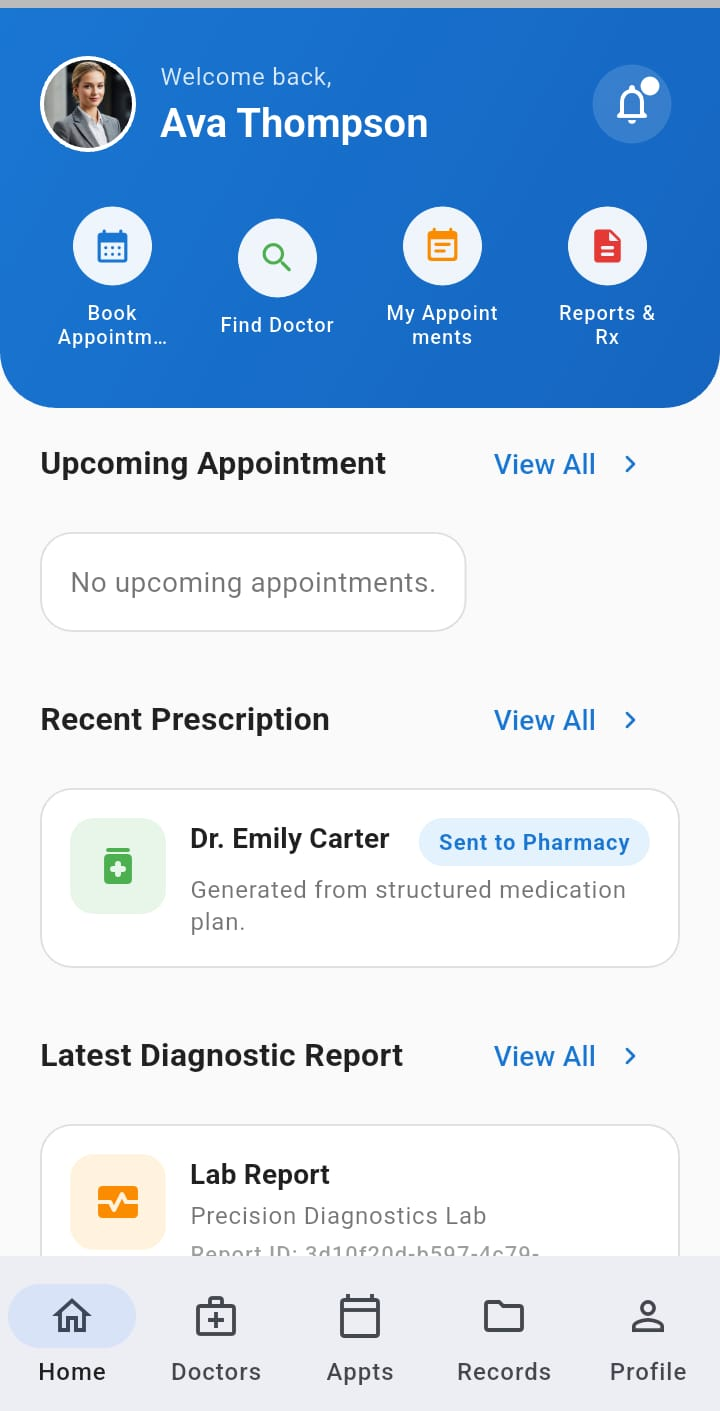
\includegraphics[height=0.62\textheight,keepaspectratio]{mobile-dashboard}
\caption{Patient Mobile Dashboard Interface}
\label{fig:mobile_dashboard}
\end{figure}

\subsection{Qualitative Results}

The React web app, Flutter android emulator, and Thunder Client were tested manually.
Role redirect, FSM transitions, notifications, uploads, downloads, and doctor analytics.
worked as expected.

\subsection{Quantitative Results}

The results of the three automated test suites are summarised in Table~\ref{tab:testresults}.
bases. The default \texttt{npm test} suite is the result of the backend; the backend \texttt{test:e2e} is the separate one.
this does not include command.

\begin{table}[tbp]
\caption{Automated Test Suite Results}
\label{tab:testresults}
\centering
\begin{tabular}{|p{5.5cm}|p{2.3cm}|p{2.3cm}|p{2.3cm}|}
\hline
\textbf{Test Category} & \textbf{Total} & \textbf{Passed} & \textbf{Failed}\\
\hline
Backend --- Jest unit tests       & 102 & 102 & 0\\
\hline
Web --- Vitest unit/component tests & 79 & 79 & 0\\
\hline
Mobile --- Flutter unit/widget tests & 75 & 75 & 0\\
\hline
\textbf{Total}                    & \textbf{256} & \textbf{256} & \textbf{0}\\
\hline
\end{tabular}
\end{table}

The same passing-test distribution is visualised in Figure~\ref{fig:test_chart}; use the table as a source of precise totals.

\begin{figure}[tbp]
\centering
\begin{tikzpicture}[
  x=1cm,
  y=0.045cm,
  bar/.style={fill=gray!45, draw=black},
  axis/.style={black, thick},
  label/.style={font=\small},
  value/.style={font=\small\bfseries}
]
  \draw[axis] (0,0) -- (10,0);
  \draw[axis] (0,0) -- (0,120);

  \foreach \y/\text in {0/0,25/25,50/50,75/75,100/100} {
    \draw (-0.08,\y) -- (0,\y);
    \node[label, anchor=east] at (-0.15,\y) {\text};
    \draw[gray!25] (0,\y) -- (9.4,\y);
  }

  \draw[bar] (1,0) rectangle (2.3,102);
  \draw[bar] (4,0) rectangle (5.3,79);
  \draw[bar] (7,0) rectangle (8.3,75);

  \node[value] at (1.65,108) {102};
  \node[value] at (4.65,85) {79};
  \node[value] at (7.65,81) {75};

  \node[label] at (1.65,-10) {Backend};
  \node[label] at (4.65,-10) {Web};
  \node[label] at (7.65,-10) {Mobile};

  \node[label, rotate=90] at (-0.95,60) {Passed Tests};
  \node[label] at (4.7,-22) {Codebase};
\end{tikzpicture}
\caption{Distribution of Passing Automated Tests Across Codebases}
\label{fig:test_chart}
\end{figure}

\subsection{Objective Achievement}

Each of the eight goals in Chapter~\ref{chap:introduction} was achieved: five-role authentication, appointment,
prescription and lab-order FSMs, PDF and Cloudinary workflows, Authenticated WebSocket.
React dashboards, role dashboards, and the Flutter patient app as well as audit logging.
significant state changes.

\section{Conclusion}

The deployment shows that a NestJS and Prisma backend, with both a(s).
Can be react SPA and a Flutter mobile client using a shared WebSocket and REST API.
capable of modeling and implementation of the complicated role and lifecycle necessities of a real-world.
delivery of outpatient care situation.

% ============================================================
%  CHAPTER V -- SOCIETAL, HEALTH, ENVIRONMENT, SAFETY,
%               ETHICAL, LEGAL AND CULTURAL ISSUES
% ============================================================
\chapter{Societal, Health, Environment, Safety, Ethical, Legal and Cultural Issues}
\label{chap:societal-issues}

\section{Intellectual Property Considerations}

The project is built using the assistance of open-source tools that are free of charge like \texttt{NestJS}, \texttt{Prisma}, \texttt{React}, and so on.
\texttt{PostgreSQL}, \texttt{PDFKit}, \texttt{Flutter}, and \texttt{Socket.IO}. \texttt{Cloudinary} SDK, and IO. No proprietary third-party
real patient/code was involved; the codebase of the project is original work by the author.

\section{Ethical Considerations}

The system handles sensitive health records such as medical records, diagnoses, etc.
prescriptions, and diagnostic results. It utilises data minimisation, hash passwording using \texttt{bcrypt}.
audit logging, role based access and secure password reset codes, hashed and expiring,
bleeding bounds and state protection.

\section{Safety Considerations}

Input validation and FSM validators are implemented with the help of DTO decorators in order to prevent clin-
JWT sends tokens to invalid \texttt{Socket.IO}, iconically nonsense states. clients are
not connected, \texttt{Prisma} (parameterizes database queries) and \texttt{Cloudinary} uploads are \texttt{HMAC-}
\texttt{SHA256} signed.

\section{Legal Considerations}

Production deployment would be required in Bangladesh that would comply with the Digital.
Security Act 2018. There would also be the need of functions to deployments of European Union residents.
GDPR-aligned erasure, portability, retention and privacy practices. The full compliance would also involve rest encryption, privacy notice, retention/deletion policy and data.
protection assessment.

\section{Impact of the Project on Societal, Health, and Cultural Issues}

Appointment in real-time will help MedFlow to avoid the waiting-room long queues.
enhance, decreases losses in prescriptions or misinterpretation by making them digital, and minimises.
drive to gather lab report. It also follows the Bangladeshi definition of family involvement by.
bringing appointment and result to a personal device.

\section{Impact of Project on the Environment and Sustainability}

The use of paper is reduced by electronic booking, prescriptions and diagnoses.
unnecessary travel. Cloud hosting can also reduce idleness in infrastructure pretty much compared with dedicated.
on-premise servers, and making healthcare administration less environmentally-intensive.

% ============================================================
%  CHAPTER VI -- COMPLEX ENGINEERING PROBLEMS AND ACTIVITIES
% ============================================================
\chapter{Addressing Complex Engineering Problems and Activities}
\label{chap:complex-engineering}

\section{Complex Engineering Problems Associated with the Current Project}

Numerous intricacies were addressed. The appointment, prescription and First.
FSMs lab ordered were needed to perform transition validation and to do other side effects such as notification.
leave This leaves no trace with PDF generation, \texttt{Cloudinary} upload and audit logging.
Second, the WebSocket gateway was supposed to have secure reconnection behaviour, which was taken care of with the usage of JWT-
authenticated per-user rooms. Third, the state of the authentication had to conform in the Flutter application.
via navigation and real-time events, processed with a \texttt{SessionController} monitored.
by \texttt{GoRouter}. Fourth, the \texttt{Appointment} was a relation that had to be named in \texttt{Prisma}.
\texttt{Appointment} refers To patient and physician.

\section{Complex Engineering Activities Associated with the Current Project}

The project included evolution of a database; 15 \texttt{Prisma} migrations.
\texttt{Cloudinary} \texttt{PDFKit} Buffers \texttt{PDFKit} Buffers and \texttt{Cloudinary} Uploads \texttt{PDFKit} PDF pipeline over JSON medication data.
stored document URLs, a layered Flutter model with maps, repositories, models,
and controllers. \texttt{React}/\texttt{Vitest} role-flow tests and testing had to be mocked as well by backend \texttt{Jest}.
\texttt{Flutter} unit/widget tests.

% ============================================================
%  CHAPTER VII -- CONCLUSIONS
% ============================================================
\chapter{Conclusions}
\label{chap:conclusions}

\section{Summary}

MedFlow: An Integrated Out-, was designed, implemented and evaluated in this project.
Connecting Patient Care. The server in \texttt{NestJS}/\texttt{Prisma}/\texttt{PostgreSQL} is an implementation of.
10 examples, 5 roles, appointment/prescription/lab FSMs, Web Socke notifications, PDF.
generation, Cloudiny storage, audit logging and password reset. The \texttt{React} web frontend.
provides job-specific dashboards and workflows, and the \texttt{Flutter} UI provides a mobile experience.
the patient experience of scheduling doctor visits, prescription and lab visits.
reports. The certified automated suites fulfilled 256 backend, web and mobile tests.

\section{Limitations}

The YouToPhone application now has five major limitations: the mobile application only has.
totients; Redis-prohibited sockets and load.IO Scaling has not been done; no certified.
OWASP Top 10 security audit has been deployed; email delivery is just a prototype stub;
and appointments are not in yet reserving slots on availability of doctors.

\section{Recommendations and Future Works}

{\looseness=-1
The mobile assistance to the doctor, pharmacy and diagnostic functions must be extended into the future,
add a \texttt{Socket.IO} Redis email adapter, an email production service.Validate, and scale-out.
request of appointment in case of unavailability of doctors. \texttt{WebRTC} are other extensions.
teleconsultation, an Admin audit dashboard, connection with the national patient identifier, ML-
no-show/specialist/prescription analysis assistants, formal audit of security and privacy assistant.
before actual practice with patients.\par}

% ============================================================
%  REFERENCES
% ============================================================
\clearpage
\begingroup
\renewcommand{\bibname}{References}
\setstretch{1.2}
\begin{thebibliography}{99}
\setlength{\itemsep}{6pt}
\setlength{\parsep}{0pt}

\bibitem{r1}
Bates, D.~W. and Gawande, A.~A., 2003, ``Improving Safety with Information Technology,''
\textit{New England Journal of Medicine}, Vol.~348, No.~25, pp.~2526--2534.

\bibitem{r2}
Shortliffe, E.~H. and Cimino, J.~J. (Eds.), 2014, \textit{Biomedical Informatics:
Computer Applications in Health Care and Biomedicine}, 4th ed., Springer, New York.

\bibitem{r3}
Richardson, L. and Ruby, S., 2007, \textit{RESTful Web Services}, O'Reilly Media,
Sebastopol, CA.

\bibitem{r4}
Hossain, M.~S. and Ahmed, F., 2019, ``Challenges of Healthcare Information Systems in
Bangladesh,'' \textit{International Journal of Healthcare Information Systems and
Informatics}, Vol.~14, No.~2, pp.~1--15.

\bibitem{r5}
Kamrul, I. and Rahman, M., 2021, ``A Review of Appointment Scheduling Systems for
Outpatient Clinics in South Asia,'' \textit{Journal of Health Informatics in Developing
Countries}, Vol.~15, No.~1, pp.~45--60.

\bibitem{r6}
Witten, I.~H. and Frank, E., 2011, \textit{Data Mining: Practical Machine Learning
Tools and Techniques}, 3rd ed., Morgan Kaufmann, Burlington, MA.

\bibitem{r7}
Mamlin, B.~W.\ \textit{et al.}, 2006, ``Cooking Up an Open-Source EMR for Developing
Countries: OpenMRS --- A Recipe for Successful Collaboration,'' \textit{AMIA Annual
Symposium Proceedings}, pp.~529--533.

\bibitem{r8}
Bowen, W., 2007, ``OpenEMR: An Open-Source Electronic Medical Record Application,''
\textit{Linux Journal}, Vol.~2007, No.~158, pp.~2.

\bibitem{r9}
Fielding, R.~T., 2000, \textit{Architectural Styles and the Design of Network-based
Software Architectures}, Ph.D. dissertation, University of California, Irvine.

\bibitem{r10}
Kaminsky, D. and Shah, R., 2022, ``NestJS in Enterprise Healthcare Backends: A
Systematic Review,'' \textit{IEEE International Conference on Software Engineering},
pp.~112--119.

\bibitem{r11}
Bui, T.~A. and Nguyen, H.~T., 2021, ``Flutter-Based Telemedicine and Appointment
Applications: Design Patterns and Challenges,'' \textit{International Journal of Mobile
Computing and Multimedia Communications}, Vol.~12, No.~3, pp.~18--34.

\bibitem{r12}
Prisma, 2023, ``Prisma ORM Documentation,'' Available online:
\texttt{https://www.prisma.io/docs}, Accessed: December 2023.

\bibitem{r13}
NestJS, 2023, ``NestJS Documentation,'' Available online: \texttt{https://docs.nestjs.com},
Accessed: December 2023.

\bibitem{r14}
Flutter, 2023, ``Flutter Documentation,'' Available online: \texttt{https://docs.flutter.dev},
Accessed: December 2023.

\end{thebibliography}
\endgroup

\end{document}
